\documentclass[onecolumn, draftclsnofoot,10pt, compsoc]{IEEEtran}
\usepackage{graphicx}
\usepackage{url}
\usepackage{setspace}
\usepackage{listings}


\usepackage{geometry}
\geometry{textheight=9.5in, textwidth=7in}

% 1. Fill in these details
\def \CapstoneTeamName{		Nexusphere}
\def \CapstoneTeamNumber{		48}
\def \GroupMemberOne{			Meghan Mowery}
\def \GroupMemberTwo{			Louis Duvoisin}
\def \GroupMemberThree{			Sarahi Pelayo}
\def \CapstoneProjectName{		A-Frame Live Stream Portal}
\def \CapstoneSponsorCompany{	Oregon State University}
\def \CapstoneSponsorPerson{		Behnam Saeedi}

% 2. Uncomment the appropriate line below so that the document type works
\def \DocType{		Project Hand Off
				%Requirements Document
				%Technology Review
				%Design Document
				%Progress Report
				}
			
\newcommand{\NameSigPair}[1]{\par
\makebox[2.75in][r]{#1} \hfil 	\makebox[3.25in]{\makebox[2.25in]{\hrulefill} \hfill		\makebox[.75in]{\hrulefill}}
\par\vspace{-12pt} \textit{\tiny\noindent
\makebox[2.75in]{} \hfil		\makebox[3.25in]{\makebox[2.25in][r]{Signature} \hfill	\makebox[.75in][r]{Date}}}}
% 3. If the document is not to be signed, uncomment the RENEWcommand below
%\renewcommand{\NameSigPair}[1]{#1}

%%%%%%%%%%%%%%%%%%%%%%%%%%%%%%%%%%%%%%%
\begin{document}
\begin{titlepage}
    \pagenumbering{gobble}
    \begin{singlespace}
    	%\includegraphics[height=4cm]{coe_v_spot1}
        \hfill 
        % 4. If you have a logo, use this includegraphics command to put it on the coversheet.
        %\includegraphics[height=4cm]{CompanyLogo}   
        \par\vspace{.2in}
        \centering
        \scshape{
            \huge CS Capstone \DocType \par
            {\large\today}\par
            \vspace{.5in}
            \textbf{\Huge\CapstoneProjectName}\par
            \vfill
            {\large Prepared for}\par
            \Huge \CapstoneSponsorCompany\par
            \vspace{5pt}
            {\Large\NameSigPair{\CapstoneSponsorPerson}\par}
            {\large Prepared by }\par
            Group\CapstoneTeamNumber\par
            % 5. comment out the line below this one if you do not wish to name your team
            \CapstoneTeamName\par 
            \vspace{5pt}
            {\Large
                \NameSigPair{\GroupMemberOne}\par
                \NameSigPair{\GroupMemberTwo}\par
                \NameSigPair{\GroupMemberThree}\par
            }
            \vspace{20pt}
        }
        \begin{abstract}
        % 6. Fill in your abstract    
        	A-Frame Live Stream Portal is a project that will be used to bring families closer together, even when adversity keeps them apart. This report is a collection of all of the major documents that were created during the year for this project. 
        \end{abstract}     
    \end{singlespace}
\end{titlepage}
\newpage
\pagenumbering{arabic}
\tableofcontents
% 7. uncomment this (if applicable). Consider adding a page break.
%\listoffigures
%\listoftables
\clearpage

% 8. now you write!
\section{Introduction to Project}
    \subsection{Introduction}
    \IEEEPARstart{T}{he} supreme court decided in a 5-to-4 vote to support President Trump`s travel ban and restrictions on people from Iran, Libya, North Korea, Somalia, Syria, Venezuela and Yemen traveling into the United States of America [1]. 
    It is estimated that one million Iran American citizens live in the United States. 
    The number is so high because Iran produces more visas than the other countries. 
    The issue now comes when relatives in Iran want to visit their families in America.
    Jamal Abdi, vice president of policy at the national Iranian American Council, points out that, to travel, Iranians must go through an unpredictable process to obtain a waiver [1]. 
    The uncertainty of obtaining the waiver makes it almost impossible for Iranian people to travel to the United States for the time being. 
    Behman Seedi's family would like to attend his wedding, however their travel plans are disrupted by the improbable chance of getting past the travel ban. 
    To accommodate for them not being there physically, our sponsor wishes to create a system where the family can still view the wedding.
    The main problem that we will be solving is giving an immersive, and complete experience while also considering distance, and efficiency.
    Since the sponsor's family lives in another country, we will need to research possible issues with bandwidth, delay during live streaming, and time-zone differences.
    We also need the solution to be efficient or else the family might miss an important part of the wedding due to a delay in the streaming.
    Another problem that will have to be solved is the possibility of a delay between audio and visual output. 
    This delay would make the experience not as enjoyable for a viewer as it could be challenging to understand what is happening during the ceremony if the audio is not in sync with the video.
    To solve this problem, the sponsor suggests that we create an interactive web portal. 
    Wedding preparation is stressful, so we will need to make the project simple enough so the sponsor is not stressed about the project. 
    \newline 

    \subsection{Solution}
    Our desire is to create a system that is more interactive than traditional forms of wedding videography and photography.
    Normal wedding pictures and video need to be edited which can take days and relatives will have missed the events taking place.
    To include our sponsor's absent family, the wedding will instead be streamed live. 
    The solution for this problem is combining a web portal with various cameras that the relatives can select which will allow them to view the proceedings.
    We will create an attractive website with an intuitive interface which will allow those tuning in to explore the venue using a complete map by clicking on the device icons. 
    The map must also have an edit mode which gives it the capability of being updated, letting the camera's locations be moved to different parts of the venue, as well as giving it the option to add or remove cameras at will.
    The web portal will need to be simple and easy to understand so usability does not become an issue for the family viewing the wedding.
    The web portal will be developed using Linux as the operating system, Apaches as the web server, MySQL as the relational database, PHP as the scripting language, and Javascript in conjunction with a Mozilla A-Frame as a framework for handling the 360 video stream. 
    \newpage
    
    Another part of the solution will be the cameras themselves; we want to make them sturdy to reduce the risk of them falling over and breaking. 
    The cameras will broadcast to a website that will be streaming everything in real time at a minimum of three locations. 
    One of the cameras will also have 360 degree video streaming capability that will provide the relatives an even more immersive experience than looking at wedding photos days later.  
    The streaming devices will be positioned around the venue and will have their own internet connection so that they can stream their video feed.
    Therefore these cameras will also need their own WiFi modules and work independently.
    The cameras will have at least 1080p at 30fps stream quality, they will also need to be portable, and easy to set up.
    The ideal choice would then be to use batteries to allow for ease of use and, being portable, we would not be able to have any type of wires connected to them.
    The batteries will either need to be easily swappable, or be large enough to power the cameras for the entire duration of the wedding ceremony.
    Our hope is that the family will have an enjoyable experience that they would not be able to have in other circumstances.

    \subsection{Performance Metrics}
    The complete project will be separated into two parts, one hardware and one software.
    To capture the wedding experience a minimum of three portable streaming devices will be deployed at the venue. 
    Our project will be considered complete when we are able to connect at least 3 cameras to our server, have them stream video to the server, and have the server hosting a website that users can connect to and select a stream to view. 
    The website's map will have the physical location of the devices as clickable icons linking to a separate page where users are able to view the stream. 
    When a device is clicked, a 480p and 30 frame per second stream will be opened in the new page. 
    The map’s interface will have an edit mode that allows for the update of the venue map image using a .png or .jpeg. 
    Because the streaming devices are independent, the edit mode will also have the options to add, remove, and reposition devices on the map which can be saved. 
    All of the cameras will need to be able to record at 1080p and 30 frames per second, and one of the cameras will also need to broadcast in 360 degree video.
    The cameras and microphone will be portable and easy to set up so they can be moved to and from sites as well as within the venue. 
    All of the cameras will be independent from one another and be broadcasting to our web portal though the use of independent WiFi modules. 
    \\
    \\
    The project itself will need to be fully functional and be usable by the sponsor and their family, and this means that we will have to complete various tests throughout the creation of the project to make sure that the finished product meets the sponsor's standards.
    To check that the product meets the sponsor's standards, we will be conducting usability tests with Jenna after the project is running to make sure the interface is accessible to those with less technical expertise. 
    We most likely will include a test run with the family so we can make sure the product is tested as it would be used on the wedding day. 
    We hope to also make the cameras themselves visually attractive so they do not take away from the overall appearance of the wedding. 
    If we complete all of the necessary parameters with enough time for the deadline, we will work to make the experience even more enjoyable for the family. 
    These performance metrics depend on the desire of the sponsor and what they wish for us to create so their entire family can experience and enjoy this special event
\newpage
\section{Requirements Document}
\begin{center}
 \begin{tabular}{||p{1cm} p{7cm} p{7cm}||} 
 \hline
 Section & Origional & New\\ [0.5ex] 
 \hline\hline
 2.1.3.1 & Document overview & Rewording\\
 \hline
 2.1.3.1 & Functional requirements & Rewording \\ 
 \hline
 2.1.3.4 & Mentioned English and Farsi & No words on viewer page, only English for admin page \\ 
 \hline
 2.1.3.6 & Mentioned developer mode & Removed developer mode \\ 
 \hline
  2.1.3.13 & Packaging, handling... & Rewording \\ 
 \hline
 2.4 & Old Gantt chart was included & Updated Gantt chart \\[1ex] 
 \hline
\end{tabular}
\end{center}
\subsection{Introduction}
    \subsubsection{Document purpose}
    The purpose of this report is to describe in detail the work to be done on the project, and the specific functions that will need to be implemented as requested by the sponsor.

    \subsubsection{Document scope}
    This document will cover all aspects of the project, including the hardware and software development.
    The report also includes a gantt chart to show our expected completion of different aspects of the project.
    
    \subsubsection{Document overview}
    
    \paragraph{System context} \\
        The finished A-Frame Live Stream Portal will be able to livestream video from at least 3 camera devices, one of which must be 360 degree video, at 480p and 30 fps. 
        The system shall also stream audio in conjunction with the video stream. 
        Users will connect to a web portal where they are able to select on a map which device they will view the the livestream from. 
        The site owner shall also be able to modify the map and the locations of the cameras.
        The system has two major parts, the streaming devices, and the server hosting the web portal. 
        The streaming devices shall capture videos of the wedding and each will individually stream that data to the server through their own internet connection. 
        The server shall allow users to connect to the map of the venue and select a device to view the wedding from. 
        The server will then send the video coming from the selected camera to the user along with the audio.
        \\
        \paragraph{Systems Functions}\\
        The function of the cameras shall be to record the wedding live. 
        Two of these cameras will be in a regular mode, while the other has 360 degree capabilities. 
        This way, the family can have a more realistic view of the ceremony.
        The web portal shall be used to access the cameras. 
        The web portal shall display the location of the cameras to the family, and they will have the option to select a camera to use. 
        The sponsor will have the ability to edit the locations of the cameras on the web portal, as well as update the map of the venue. The sponsor will also be able to add and remove cameras as desired.
    \\
        \paragraph{User characteristics}
        The system has 2 types of users, admins and viewers. 
        Admins are the users who will set up the devices and have the ability to edit the map and location of devices on the web portal.
        Viewers will need to log in with an access token and will then be able to select a device on a map of the venue, which is also visible by admins. 
        When either a viewer or an admin clicks on a device they shall be taken to a new page with the livestream from the device they chose.

        \subsubsection{Definitions} \\
        \begin{tabular}{ll}
         Fps & Frames Per Second \\ 
         Jpeg & Joint Photographic Experts Group (image file format) \\ 
         Png & Portable Network Graphics (image file format) \\
         Web Portal & A website that displays information from multiple external sources \\ 
         Access Token & Randomly generated sequence of characters used for authentication \\
        \end{tabular}

\subsection{System requirements}
    \subsubsection{Functional requirements}
    This system is being developed to allow the relatives of our sponsors to experience our sponsors' wedding from outside of the country.
    Two cameras shall stream normal video from two locations to the web portal a third camera shall also stream 360 degree video to the web portal. In addition to the three cameras, audio will also be streamed with the video.
    The web portal shall run properly without crashing even when devices are added or removed.
    
    \subsubsection{Usability requirements}
    Each streaming device will have their own internet connection so that they can stream their video feed independently of one another.
    The web portal will broadcast the video with a maximum of one minute delay. Changing the battery of the devices will be quick and easy to do. 
    
    \subsubsection{Performance requirements}
    The cameras will have at least 480p at 30fps stream quality with the maximum latency of one minute. 
    Each camera with a fully charged battery will last at least the average time of a wedding ceremony. 
 
    \subsubsection{System interface}
    The system will have an attractive website with an intuitive interface which will allow those tuning in to explore the venue using a complete map by clicking on the device icons. 
    The website's map will have the physical location of the devices as clickable icons linking to a separate page where users are able to view the stream.
    The map's edit mode shall mainly use symbols for adding, removing, and updating the location of cameras. Words on the website will be kept to a minimum and are only present in admin mode.

    \subsubsection{System operations}
    The web portal will have a log-in page, where the user will enter a code given to them by the sponsor.
    Both users and admins will log in using access tokens, if we have enough time to implement it admins may instead log in using a username and password.
    Visitors can select an image (one representing either the normal or 360 view camera) to view that devices stream. 
    The admin can also add and remove cameras, as well as update the web portal's map.
    The cameras can be powered on and off, and have independent WiFi connections meaning if one fails the system can continue uninterrupted. The cameras will need to be connected to WiFi at the venue.
    
    \subsubsection{System modes and states}
    The system will have two modes: normal and edit. The map’s interface will have an edit mode that allows for the update of the venue map image using a .png or .jpeg. 
    Because the streaming devices are independent, the edit mode will also have the options to add, remove, and reposition devices on the map which can be saved. The normal mode will be what viewers use where they can interact with the map and access streams.
    
    \subsubsection{Physical characteristics}
    %needs to be rain proof
    The hardware shall be encased so there are no exposed wires while buttons will still remain accessible.
    The cameras themselves will be sturdy to reduce the risk of them falling over and breaking however weighing no more than 20lbs each. 
    The battery will be removable.
    The web portal will be as simplistic as possible.
    This means that the web portal will have limited words, and instead use icons to represent the different functions of the system. Although the system is being developed for three cameras the system may have the option for expanding the system with more cameras.
    The system is not water resistant but will be rain proof.
    
    \subsubsection{Environmental conditions}
    The hardware is expected to preform well in conditions that are considered suitable for humans between 15 degrees Celsius to 25 degrees Celsius. 
    The system shall work well in indoor conditions. Performance and quality may be affected by lighting, wind, extreme temperatures, flora, fauna, fungus, mold, sand, salt spray, dust, radiation, chemical, immersion, motion, and shock.
    
    \subsubsection{System security}
    The owner will be admin by default. 
    Only admins will be allowed to enter edit map mode. 
    Viewers will not be allowed to change locations, add, or remove devices on the website's map. 
    To respect the privacy of users, streams will be private. 
    Viewers will be able to log in with an access token to access the broadcasts. Users will agree that their private streams may be accessed by developers for troubleshooting but will not be shown to the general public.
    
    \subsubsection{Information management}
    The system will store the generated tokens used for viewers to log-in to the web portal.
    The audio and video recorded from the wedding will be live streamed directly to the viewers.
    
    \subsubsection{Policies and regulations}
    The system will maintain the privacy of the viewers and attendees of the wedding through the information listed in section 2.2.9.
    
    \subsubsection{System life cycle sustainment}
    To sustain the system, the cameras will need charged batteries, and the computers accessing the web portal will also need a reliable internet connection. 
    In case of a camera failure or breakdown, the web portal contains an option to add or remove cameras from the system so they can be replaced if needed.
    Basic understanding of the web portal and the cameras will be required to maintain and utilize the system.
    
    \subsubsection{Packaging, handling, shipping and transportation}
    The cameras and microphone will be portable and easy to set up so they can be moved to and from sites as well as within the venue. 
    The hardware of the systems shall be packages with shock absorbing material and labeled as fragile. 
    When shipping the packaged system it shall be handled gentle as to not destroy an part. 
    
\subsection{Verification}
The system will be considered fully operational when the web portal is operational by both the admin and the viewers, and the cameras properly record and stream the video and audio.
The admin will be able to edit the display of the web portal, including the cameras, as desired.
Finally, the viewers will be able to access the portal with their distributed tokens to view the ceremony.

\subsection{Gantt Chart}
\begin{figure}[h]
    \centering
    \includegraphics[width=0.8\linewidth]{Images/gantt_chart.png} 
    \caption{Gantt chart showing the time line of our project.}
\label{fig1}
\end{figure}
\newpage
\section{Design Document}

\begin{center}
 \begin{tabular}{||p{1cm} p{7cm} p{7cm}||} 
 \hline
 Section & Original & New\\ [.5ex] 
 \hline\hline
 3.1.3 & Had 720p as resolution & Lowered to 480p\\
 \hline
  3.1.3 & Microphone was originally going to be it's own separate pi & Microphones now attached to all pis\\
   \hline
  3.3.2 & Had one microphone & Now uses three microphones\\
  \hline
  3.3.3.1 & Referenced using a UML diagram & Removed references\\ 
  \hline
  3.3.3.2 & Referenced using a UML diagram & Removed references\\ 
  \hline
  3.3.3.3 & Microprocessor section & Removed section, no longer using microprocessor  \\
  \hline
  3.3.3.3/4 & Mentioned using 1 microphone & Now using 3 microphones \\
    \hline
 3.3.4.1 & Mentioned microprocessor & Removed microprocessor reference and added a microphone per pi \\
  \hline
 3.3.4.1 & VLC was going to be used for streaming & Picam and a node plugin were used instead \\ 
 \hline
 3.3.4.1 & MJPEG was the original file format & HLS is what was used\\ 
 \hline
 3.3.4.2 & 360 video camera was going to be purchased & The raspberry pi camera module with a 360 degree lens attachment was used\\
 \hline
 3.3.4.3 & Section talking about microprocessor & Removed section \\ 
 \hline
 3.3.4.3/4 & Microphone design was using one microphone and a microprocessor to merge audio & New design has a microphone on every pi creating a stream with audio \\ 
 \hline
 3.3.4.4/5 & Section references the ad hoc network & Revisions regarding the ad hoc network\\
 \hline
 Figures & Old pictures of prototypes & New pictures of the current appearance of the website\\[1ex] 
 \hline
\end{tabular}
\end{center}

\subsection{Introduction}
    \subsubsection{Purpose}
    The purpose of this document is to describe the different physical aspects of this project.
    By describing the aspect of the project in detail, it will be easier to formulate a plan to complete the project.
    This includes describing the design concerns, views, and viewpoints of this project.
    
    \subsubsection{Scope}
    This document will cover all aspects of the project, including the hardware and software development.
    This document also includes various images related to the system's user interface and design.
    
    \subsubsection{Context}
    A-frame live stream portal is a project that will utilize various technologies to allow the stakeholder's family to view the stakeholder's wedding live.
    The project consists of three cameras, two regular view and one 360 view which will be live streaming the wedding at 480p and 30fps. 
    Each raspberry pi will have a microphone attached which will provide audio for the stream coming from that pi.
    Finally, the web portal that will be created will be used by both the stakeholder and the stakeholder's family.
    The stakeholder will have access to an admin page where they can move, add, or delete cameras and microphones as well as change the displayed venue map.
    The users will be able to select any of the available cameras on the map to view the wedding ceremony.
    This way the family of the stakeholder will be able to experience the wedding as if they were there themselves
    %\begin{table}[H]
    %\caption{Glossary}
\subsection{Glossary}
    \begin{tabular}{l5}
             Access Token/Login Key & Sequence of characters used for authentication \\
             A-Frame & The web framework that will be used for 360 video \\
             CSS & Cascading Style Sheet\\
             Fps & Frames Per Second \\ 
             Jpeg & Joint Photographic Experts Group (image file format) \\ 
             Mbps & Mega bits per second \\
             Mjpeg & Motion Joint Photographic Experts Group 720p \& Progressive video format with 720 horizontal lines\\
             Png & Portable Network Graphics (image file format) \\
             TCP & Transmission Control Protocol\\
             UDP & User Datagram Protocol \\
             USB & Universal Serial Bus\\
             UI & User interface \\
             Server & The computer hosting the website and receiving the video\\ 
             Web Portal & A website that displays information from multiple external sources \\ 
             Wi-fi & Wireless Fidelity
    \end{tabular}
    %\end{table}

\subsection{Body}

    \subsubsection{Identified design stakeholders}
    The stakeholders for this project are Behnam and Jenna Saeedi.
    
    \subsubsection{Identified design concerns}
    This project will require both a user interface (UI) and technological implementation.
    The web portal will have two different interfaces, admin and user, and will be simple and easy to understand.
    The technologies used for this project will be two video cameras, one 360 degree video camera, three microphones, and multiple raspberry pis.
    
    \subsubsection{Selected design viewpoints}
    %identifies the design concerns to be focused upon within its view and selects the design languages used to record that design view
        \paragraph{Normal Video}
        The video needs to be live streamed from the wedding to the stakeholder's family.
        This video will ideally stream at 1080p and 30fps with a minimum of 480p, still with 30fps.
        The stream can be interacted with by the stakeholder's family.
        The camera will need to last the entire wedding ceremony.
        
        \paragraph{360 Video}
        The 360 video needs to be live streamed from the wedding to the stakeholder's family.
        This video will ideally stream at 1080p and 30fps, and can be interacted with by the stakeholder's family.
        The camera will need to have a strong enough battery so it can last the entire wedding ceremony.
        
        %\subsubsection{Microprocessor}
        %The microprocessor has to have the capability to stream either the regular or 360 degree video to the web portal without any significant delays. 
        
        \paragraph{Microphone}
        To get the full experience of the wedding for the family of the client along with streaming video there will be audio to accompany it. The system’s design includes three cameras and three microphones. Because each raspberry pi will have its own microphone attached, each stream will have its own audio feed.  
        A subsystem is a camera or microphone connected to a microprocessor. 
        The goal of the microphones are to record and stream audio so it can be projected over the each video broadcast coming from the other raspberry pis. 
        
        \paragraph{Web Server Architecture}
        The web server architecture must be designed so all the video and audio streams from the four subsystems can be sent to a web server. 
        The network design must allow for subsystem independence, meaning that if one of the cameras fails the others must remain unaffected.  
        %probably have images showing how our technologies will be used
        %IE: front end/back end/hardware
        %UI & Video Player/Web Host/Streaming device & Camera
        
        \paragraph{Desktop UI}
        The user interface needs to be designed in a way that is simple to use for both the client and the end user. 
        A custom website will be designed. The website's UI will be tailored with input from the client.  
        The design will go through a feedback process where a prototype will be presented to the client, and the client will leave feedback as they see fit. 
        After the client's feedback the prototype will be updated and shown to the client again. 
        The web page will require users to login to view the venue map, and be able to select a device from a camera to watch the wedding. 
        Users will also need to be able to return back to the venue map and select a different device. 
        There will also be an admin view from which the client can add, move, and remove cameras, as well as upload a new venue map.
        
        \paragraph{Mobile UI}
        In addition to working on desktop, the website will also need to be usable on mobile devices. 
        All functionality available in the desktop UI must be available for mobile.
        
    \subsubsection{Design views}
    %Each view addresses a specific set of design concerns of the stakeholders
        \paragraph{Normal Video}
        Video in normal view will contain two subsystems consisting of a raspberry pi camera module and microphone. 
        The module with be connected to the raspberry pi's camera port using a ribbon cable. 
        For video streaming, the design will need a video media player. 
        Picam will be used to record the stream and a node app will act as the server for the stream because it has several options to customize the stream so it can meet the requirements of a minimum of 480p with 30fps. 
        The video will be in HLS format and adjusted to a reasonable bit rate at will depend on the strength of the venue's Wi-Fi. 
        
        \paragraph{360 Video}
        The 360 video stream will be done with a basic raspberry pi camera module and an additional attachment that is used for streaming 360 video on iPhone, the user will connect the pi and operate it the same way they would operate the regular videos on the raspberry pi.
        The video will then be streamed to the website using A-Frame.
        The team chose to upload the video directly to the website instead of going through another format such as YouTube or Facebook.
        
        \paragraph{Microphone}
        The best design approach selected will be to have a microphone connected to each raspberry pi.  
        The independence of the mentioned design choices meets the need for safeguarding from total system failure as a result from one competent or subsystem failure.
        A USB microphone will be used on each raspberry pi 3 to record the audio used for each stream. 
        USB microphones have easy interfaces meaning that it can be inserted into any USB port. 
        The audio will be streamed with picam, which captures both audio and video from the attached pi. 

        
        \paragraph{Web Server Architecture}
        Each of the microprocessors need to have a built-in wifi module to be able to connect to the internet. 
        The network will consists of three subsystems, two normal video, and one 360. 
        Each microprocessor will send captured video and audio to the web server directly using the venue internet. 
        The raspberry pi from a will have the IP address of the venues router then the router will port forward to the pi. The video will be port forwarded from each of raspberry pi to the router then sent over to the OSU server.This architecture is illustrated in Figure 11.

        \paragraph{Desktop UI}
        Figure \ref{fig:Login} is the login page of the system's website. Users will be given a login key which they will input. When the user's enter the correct key they will be taken to the main page, Figure \ref{fig:User}. The main page is where users will be able to select which stream they want to watch. The main page also has an admin view shown in Figure \ref{fig:Admin}. The client will be able to get to admin view by logging in with a separate login key for the admin login. The buttons will open menus that will allow the client to perform the labeled action (ex: add a device, remove a device, etc). In both admin and normal user mode clicking on a camera will redirect the user to that camera's stream viewable in Figure \ref{fig:Video}. The video page will be the same for both normal and 360 video.

        \paragraph{Mobile UI}
        The mobile UI will contain the same pages as the desktop UI and have all of the same functionality. The system's CSS will be written such that the user will be loading what would be the same page both on desktop and mobile, but the page's components for the mobile view will be oriented differently. Figure \ref{fig:MLogin} through \ref{fig:MVideo} are the mobile versions of the pages talked about in the Desktop UI section
\newpage
\section{Tech Review}

    \subsection{Louis}
    
        \subsubsection{What we're trying to accomplish}
        We are trying to live stream our sponsor's wedding to his family in Iran who can not attend due to the travel ban put in place by the current administration. In order to do this we need multiple different technologies. In this document I will be introducing multiple options for our UI, multiple options for the cameras our devices will have, and multiple methods for connecting our devices to the internet.
        
        \subsubsection{UI Frameworks}
            UI Frameworks, while not a necessity, make starting a project much easier. Frameworks provide a starting block to build your website off of, and provide many pre-styled components for developers to use. In this section I will be assessing different frameworks on: customizability, size, difficulty of setup, and difficulty to work with.
            \paragraph{Bootstrap}
            Bootstrap is the most popular UI framework in use today \cite{IEEEhowto:Bootstrap}. It is heavily customizable and many people have already made 3rd party extensions and add-ons, which we could also use. The framework also supports mobile devices so making our site mobile friendly shouldn't be too hard. One downside of Bootstrap is that it is quite a large framework and would greatly increase the size of our project. Our website will not have many different pages, but Bootstrap is most useful for large websites with multiple components that should look identical throughout the site. Our website is going to be at most 5 pages, with very few repeated components. In addition, Bootstrap is built to use a 12 column system with percentage based sizing as opposed to the more flexible grid available with base CSS. Bootstrap is a great framework, but I think that because the website needed for our project will only be at most 5 different pages, and the fact that it is tailored to the desires a specific client make Bootstrap too much effort for too little reward.
            \paragraph{Skeleton}
            Skeleton is a lightweight framework specifically designed for smaller projects \cite{IEEEhowto:Skeleton}. It is extremely small consisting of approximately 400 lines and was built with mobile viewing in mind. It is also super easy to start using as it requires no compilation or installation, you just download the file and go. A downside for most projects would be that it is not a true framework and does not contain many styled components that other frameworks have, however for this project this is acceptable, as we will likely be making our own components anyways with input from our sponsor. While Skeleton also uses the 12 column system, it has fewer styles by default, making it easier to use another system if you want.
            \paragraph{None}
            The newly released CSS Grid system has support from every major browser except for internet explorer (which makes up almost 5 percent of users in Iran \cite{IEEEhowto:CanIUseGrid}) making it easier than ever for developers to make their own layout systems. This option would provide the most customization for our sponsor as everything would be made by scratch. This would work especially well as our web site will have very few pages with duplicate styling. The obvious downside of this option is that we would be starting from scratch. Starting with an empty page is hard and a major benefit of using a framework, even a small one, is that you already have something that you can build off of.
            \newline
            \newline
            \begin{tabular}{|l|p{4cm}|p{2cm}|p{4cm}|p{4cm}|}
                 \hline
                 Framework & Customizability & Size & Setup Difficulty & Use Difficulty \\ \hline
                 
                 Bootstrap & Has many themes to select from & Very large & Not too difficult, but does take some work & Has a learning curve \\ \hline
                 
                 Skeleton & Because it has very few pre-made styles everything is customizable & Very small, only one file & Place the file in your repository and you can use it & Very easy to use \\ \hline
                 
                 None & Very customizable because nothing is preset & N/A & No setup & You need to make your own layout which makes use more difficult\\ \hline
            \end{tabular}
        
        \subsubsection{Standard Cameras}
        Our devices will need cameras in able to capture video. Our sponsor has requested that our devices be able to stream 480p video, but would be happy to get higher quality. In this section I will be comparing different cameras on: video quality, auto-focusing capability, and ease of setup.
        %update to include multiple quality streams, raspi module supports
        
            \paragraph{AUSDOM 1080P HD USB Webcam}
            This webcam is well suited for users who are trying to get the features of a full webcam at a lower price \cite{IEEEhowto:AUSDOM1080p}. It offers 1080p video, and low light enhancement. It connects with USB 2.0 or 3.0 and as a large upside weighs less than 4.5 ounces. Some downsides to this device are that it does not have an auto-focus, meaning that the end user would need to load the live streams in order to focus the device. After the device is focused however, there would be no automatic focus adjustments as people walk in front of the device which would be an upside. A small downside of this camera is that we would need to design a special stand to attach it to our devices. The device also has a microphone and some noise canceling technology but I don't think it would be a suitable replacement for using a separate higher quality microphone.
            \paragraph{Logitech C920}
            The Logitech C920 is a slightly higher end webcam, it also supports 1080p video and has low light enhancement \cite{IEEEhowto:LogitechC920}. It also connects via USB 2.0/3.0, it weighs slightly more than the AUSDOM webcam at 5.7 ounces, but that is a negligible difference for our project. This device has auto focus technology, which would mean that the person setting up the camera would not need to focus the device and would just need to connect it and walk away. The downside to an auto focus is that if the camera is in a position where people are regularly walking in front of it, the camera will try to refocus on each person, which would look weird on the livestream. Another upside to this camera is that it has stereo microphones. A device using this camera would be able to replace a fourth device only using a microphone if placed near the main source of sound.
            \paragraph{Raspberry Pi Camera module}
            This camera would be the cheapest and easiest camera that meets all the requirements set out by our sponsor. The device can stream 1080p video, and weighs less than half an ounce, far less than the other two cameras mentioned \cite{IEEEhowto:RaspberryPiModule}. The camera connects directly to a Raspberry Pi with a dedicated cable and is specifically designed to work with Raspberry Pis. This camera could actually fit inside our casing, so we would only need to make a hole for the camera to see through to attach this camera. Additionally, there are pre-existing functions for the camera module that allow different quality video to be recorded, which would be a good backup in case the venue WiFi is not able to support the amount of data being sent. A downside to this camera is that it has a fixed focus lens. That means that the user will need to make sure to place each device an appropriate distance from the content they want the camera to film, it does however do some basic image/video balancing. Another major potential downside that Dr. McGrath brought up is that in the past Raspberry Pis have had issues with video encoding and transmission over a network, we will need to test this and will determine whether or not we will use this camera. I think that should we choose to use a Raspberry Pi and we have no encoding issues, this camera is the best option as it would be the simplest to integrate and meets all of our sponsors needs.
            \newline
            \newline
            \begin{tabular}{|l|p{3cm}|p{4cm}|p{4cm}|}
                 \hline
                 Camera & Video Quality & Auto-Focusing & Ease of Setup \\ \hline
                 
                 USDOM 1080P HD USB Webcam & 1080p & Manual Focus  & Requires driver installation \\ \hline
                 
                 Logitech C920 & 1080p & Has auto-focus built in to camera & Requires driver installation \\ \hline
                 
                 Raspberry Pi Camera module & 1080p & No focusing & No drivers required \\ \hline
            \end{tabular}
        
        \subsubsection{Connectivity method}
        There are a variety of ways that our devices will connect to the internet. In all cases our devices will be streaming from the venue to our server. This section is only about how the devices will use the venue WiFi to connect to our server. The methods will be compared by reliability, ease of setup, ease of programming.
            \paragraph{Local WiFi Network}
            Making a local WiFi network for our devices to connect to would allow for an easier set up by the end user. The devices would connect to a central hub hosting a network and and would stream all of their data through the hub to our website on the OSU servers. Picking this method would mean that the person setting up the devices would only need to connect one device to the WiFi at the venue, and would simply need to turn on the other devices and they would automatically connect to the network hosted by the central hub. The downside of this option is that it would require and extra device to function as a hub, and would be more difficult for the developers to implement.
        
            \paragraph{Local Wired Network}
            Making a local wired network for our devices would be difficult for the end user to set up, but would guarantee connectivity for all our devices. The devices would be wired to a central hub, which would either connect to the venue WiFi, or be wired in to a wall port or router. The hub would then send all of the streams to our web server to be hosted on our website. This option should only be considered if we are unable to get our devices to connect to WiFi reliably enough to stream video as it would require running wires across the venue.
        
            \paragraph{Devices Connect to Server Individually}
            Having each of our devices connect to the venue WiFi and directly stream their content to our web server would be the most robust option provided our devices can connect to the venue WiFi reliably. This option would allow the system to keep running should any device stop working. The only downside to this option is that it the person setting up the devices would need to connect each device to the internet individually, through a Bluetooth phone app we will make for our sponsors phone. Another potential downside could be that the venue WiFi is not reliable enough to handle the connection of 3 devices streaming 1080p video, which is unlikely but possible. This option is the best barring unreliable WiFi, and if given the time we may implement one of the other solutions as a back-up.
            \newline
            \newline
        \begin{tabular}{|l|p{4cm}|p{4cm}|p{4cm}|}
                 \hline
                 Method & Reliability & Ease of Setup & Ease of Programming \\ \hline
                 
                 Local WiFi Network & Cameras can go down, hub can not & Only one device to setup & Requires programming a central hub to host a network\\ \hline
                 
                 Local Wired Network & Cameras can go down, hub can not. Reliant on wires & Requires connecting devices with wires to setup & Requires programming a central hub, but will be easier than a wireless network \\ \hline
                 
                 Devices Connect Individually & Devices are independent & Requires connecting each device to the internet & Requires programming a phone app to connect devices to internet. \\ \hline
            \end{tabular}
            \newline
            \newline
        \begin{louis-techreview-bib}{References}
        
        \bibitem{IEEEhowto:Bootstrap}
        https://getbootstrap.com/
        \bibitem{IEEEhowto:Skeleton}
        http://getskeleton.com/
        \bibitem{IEEEhowto:CanIUseGrid}
        https://caniuse.com/#feat=css-grid
        \bibitem{IEEEhowto:AUSDOM1080p}
        https://www.amazon.com/Microphone-Exposure-Freestanding-Computer-Messenger/dp/B012CK43W6
        \bibitem{IEEEhowto:LogitechC920}
         https://www.logitech.com/en-us/product/hd-pro-webcam-c920
        \bibitem{IEEEhowto:RaspberryPiModule}
        https://www.amazon.com/Raspberry-Pi-Camera-Module-Megapixel/dp/B01ER2SKFS/
        
        \end{louis-techreview-bib}

    
    \subsection{Meghan}
    \subsubsection{Introduction}
	The goal of this project is to allow the sponsor's family, who lives in another country, to view the sponsor's wedding.
	The project will consist of both hardware and software elements.
	The software elements are a web portal that will have a map of the venue, and icons which, when selected, takes the user to a live stream of the ceremony at the location marked on the map. 
	The icons and map can also be updated by the web portal's admin.
	The hardware portion of the project includes three cameras, one of which will have 360 degree view capabilities, audio recording, and a device to utilize the web portal's virtual reality capabilities.
	My goal is to research three different 360 degree view cameras that could be used by our system, three different VR headsets, and three different website frameworks.
	Individual roles for the project have not been delegated, and, as a team, we strive to share the work equally.
	A-Frame Live Stream Portal is a project that contains many different facets of technology, and each one needs to be researched so we are able to select the tools that will be efficient, cost effective, and satisfy our sponsor's requirements. 
	
    \subsubsection{360 degree cameras}
    The 360 degree view camera is a requirement of the sponsor.
    This camera will allow the viewers the option to view the ceremony in a more "real world" setting.
    Originally, the camera needed to stream at 1080p at 30fps. 
    However, with a concern about processing capabilities, the speed requirement has been reduced to 480p minimum.
    Below is a collection of three different 360 degree view cameras that would operate using a Raspberry Pi or BeagleBone.
    
    \paragraph{Self-made camera} \\
    One option for a 360 degree camera is a self-created camera using the Rasberry Pi directly.
    This method would also include a small mounted camera commonly used for phones.
    This method would involve directly mounting the camera onto the Rasberry Pi, and implementing code to convert that image into a usable 360 degree video.
    While this option is by far the cheapest costing approximately \$50, problems may arise involving streaming speed and video quality.
    Tinkernut provides a website that contains the link to all needed code and instructions to create this camera[7].
    If this method proves to be unusable, there are other, more expensive, options.

    \paragraph{Camorama} \\
    A second 360 degree camera option is the Camorama The 4K Action VR & 360 Camera 64GB eMMC UPC: 853466007010.
    Camorama is a new company that was created through Kickstarter.
    This camera is available on Amazon.com for \$349, and has high reviews.
    This camera does not have any descriptions regarding its specification except that it is VR compatible. 
    Since this camera does not have much information concerning it, another option might be desired.
    
    \paragraph{360fly camera} \\
    360fly 360 HD Video Camera is another camera that is on sale on Amazon.com for \$83.95.
    The reviews for this camera are mixed, but since it is prime it can most likely be returned.
    The camera itself is advertised to be "full 360-degree video with a 1504 x 1504 resolution, 32 GB internal memory and 2+ hours of battery life", and also be "virtual reality ready" [9].
    This option however does specify as a panoramic camera.
    Another option for sale in the same location is the 360Fly 4K 64GB camera at \$372.99.
    This camera promises a 360-degree video and "provides 4K video resolution 2880 x 2880 pixels up to 30fps" [9].
    Along with a 360-degree camera, the sponsor also needs a VR headset that the family can use to view the 360 stream.

    \subsubsection{VR headsets}
    The VR headset is what will be used by the sponsor's family to view the ceremony in conjunction with the 360 degree view camera and the website framework that is chosen.
    Qualities that were researched were affordability, comfort, and usability.
    Written below are three different VR headsets that would function well with the project.
    
    \paragraph{Google Cardboard} \\
    Google Cardboard is a simple VR headset that is made out of cardboard or plastic.
    All that is needed to operate a Google Cardboard is a smartphone, and you simply place the phone into the cardboard to utilize the VR features.
    It is also the cheapest option with the cost ranging from \$15 - \$30.
    The greatest downside with it is that since it is so cheap, it does not have any additional features. 
    It is also noted that the Google Cardboard does not have any real way to block external noises, which would take away from the viewing experience.
    While the Google Cardboard is the cheapest option, it is also not the highest quality by means of user experience.
    
    \paragraph{ZEISS VR One Plus} \\
    The Zeis VR One Plus, from now on referred to as Zeis is a step above the Google Cardboard in quality as well as in price.
    The Zeis ranges from \$40 - \$100 in price, and can be found at stores such as Best Buy and Target, and is compatable with any smartphone with a screen size between 4.7 and 5.5 inches.
    The Zeis is made out of fabric and plastic instead of cardboard, so it is more comfortable, and it is also designed to be comfortably used by people who wear glasses.
    To use the headset, the user inserts their smartphone into the device after opening the desired application.
    This VR headset is equipped to perform with apps that require touch input, and allows the user to select options without taking the phone out of the headset.
    The Zeis can also use Google Cardboard apps by scanning a QR code.
    The Zeis VR One Plus is slightly more expensive then the Google Cardboard, but with that cost comes higher quality materials and a better user experience.

    \paragraph{Homido V2} \\
    The Homido V2 is another mid-priced VR headset which costs around \$50 and can be purchased at any Best Buy store.
    The Homido V2 is similar to the Zeis VR One Plus in terms of comfort and quality.
    The difference between it and the Zeis VR One Plus is that the Homido V2 offers the ability to adjust the "interocular distance and focal length for myopia and hyperopia corrections", while the Zeis VR One Plus does not [3].
    The reason that the Homido V2 offers this adjustment capability is because the device is not designed to fit glasses, and this can be seen as an inconvenience for glasses wearers, especially if multiple people were using the device at the same time.
    Users would need to continually adjust the vision of the VR headset to fit their needs.
    This problem would not occur with the Zeis VR One Plus since it allows the user to wear their glasses while using the device.
    When comparing the two devices, the Zeis VR One Plus out preforms the Homido V2 in affordability, comfort, and user inclusiveness. 
    
\subsubsection{Website Frameworks} 
    The website framework is what will be used to create a website that is VR compatible.
    Our team is looking for a framework that is easy to implement and understand so we do not need to spend much of our time creating the web portal so we can focus on more technical aspects of the project. 
    For the three different frameworks, I will be researching usability, code availability and implementation.
    
\paragraph{A-Frame} \\
    A-Frame is the most commonly used website framework, and the website framework that the sponsor has suggested for us to use.
    A-Frame uses HTML, is built upon the Web VR API, and is easy to download and implement.
    The purpose of this framework is to create a webpage with the use of LAMP that is compatible with VR.
    Their main webpage provides all the links and instructions needed to use the website framework. 
    A-Frame's main website also includes various examples to explain the implementation of their product so it is easy for users to understand.
    Although A-Frame is the most common website framework, it is far from the only one.
    
\paragraph{WebVR API} \\
    WebVR API is another website framework that is used to implement VR, and is the API that A-Frame is built upon.
    WebVR uses JavaScript to implement the desired VR experience on any web browser, which can then in part be used by a smartphone.
    Like A-Frame, WebVR's code is easily accessible to the public. 
    The current problem with using just WebVR as opposed to A-Frame is that WebVR itself seems confusing to utilize and implement.
    Unlike the clear, step-by-step instructions that were provided on the A-Frame, WebVR provides more technical explanations and code samples.
    Along with WebVR and A-Frame, there are other website frameworks that can be use to implement a VR compatible website. 
    
\paragraph{Google VR} \\
    The Google VR for IOS is like the above website frameworks, and also has accessible code and clear tutorials on the Google VR website.
    Unlike the other website frameworks, this specific Google VR website framework is only usable through Iphone 8's or newer which would require the user to own an Iphone.
    Google VR does provide other website frameworks such as one for Android Studio and Android NDK for users who have Android phones, but they are separate website frameworks.
    This restriction would not make the website user friendly, as it would restrict who could utilize the VR feature depending on the type of mobile phone that they own.
    While Google VR does provide some exciting avenues for website frameworks, the phone specifications would prevent it from being as user friendly as we require for this project.

\subsubsection{Conclusion}
    In conclusion, the best 360 degree camera would be the Raspberry Pi  self-made camera due to the simplicity and cost efficiency. 
    The best VR headset would be the ZEISS VR One Plus since it offers better quality and usability versus the cheaper alternatives. 
    Finally, the best website framework would be A-Frame because it is easy to understand and implement.
    \newpage
\begin{Meghan-techreview-bib}{References}

\bibitem{IEEEhowto:kopka}
Robertson, Adi. THE ULTIMATE VR HEADSET BUYER’S GUIDE. [online] The Verge. Available at: https://www.theverge.com/a/best-vr-headset-oculus-rift-samsung-gear-htc-vive-virtual-reality [Accessed 2 Nov. 2018].

\bibitem{IEEEhowto:kopka}
Zeiss,  Carl. Virtual reality for everyone. [online] ZEISS International. Available at: https://www.zeiss.com/virtual-reality/home.html\#faq [Accessed 2 Nov. 2018].

\bibitem{IEEEhowto:kopka}
[online] Homido. Available at: https://homido.com/homido-v2/ [Accessed 2 Nov. 2018].

\bibitem{IEEEhowto:kopka}
[online] A-Frame. Available at: https://aframe.io/ [Accessed 2 Nov. 2018].

\bibitem{IEEEhowto:kopka}
Pannase, Maithili. WebVR API VS. A-Frame: What's the difference?. [online] Empact Labs. Available at: http://empactlabs.co/webvr-api-vs-a-frame-whats-the-difference/ [Accessed 2 Nov. 2018].

\bibitem{IEEEhowto:kopka}
(2018). Quickstart for Google VR SDK for iOS. [online] Google VR. Available at: https://developers.google.com/vr/develop/ios/get-started [Accessed 2 Nov. 2018].

\bibitem{IEEEhowto:kopka}
How to make a cheap 360 video camera with a Raspberry Pi. [online] Tinker Nut. Available at: http://www.tinkernut.com/portfolio/make-cheap-360-video-camera-raspberry-pi/\#lightbox[10210]/0/ [Accessed 2 Nov. 2018].

\bibitem{IEEEhowto:kopka}
[online] Available at: https://www.amazon.com/Camorama-Action-360\%C2
\%B0-Camera-64GB/dp/B01MYXP52N/ref=sr\_1\_5?rps=1\&ie=
UTF8\&qid=1541209278\&sr=8-5\&keywords=360+cameras\&refinements=p\_72
\%3A2661618011\%2Cp\_85\%3A2470955011 [Accessed 2 Nov. 2018].

\bibitem{IEEEhowto:kopka}
[online] Available at: https://www.amazon.com/360fly-360\%C2
\%B0-HD-Video-Camera/dp/B00XAIT0PU/ref=sr\_1\_1?rps=1\&ie=UTF8
\&qid=1541211154\&sr=8-1\&keywords=360+cameras\&refinements=p\_89\%3A360fly\%2Cp\_85\%3A2470955011 [Accessed 2 Nov. 2018].

\end{Meghan-techreview-bib}



    \subsection{Sarahi}
        \subsubsection{Introduction}
        The complete project will be separated into two parts, one hardware and one software.
        To capture a wedding experience four portable streaming devices will be deployed at the venue and connected to our server. They will stream video and audio to the server. From the server a a website will be hosted that users can connect to and select a stream to view. 
        The website's map will have the physical location of the devices as clickable icons linking to a separate page where users are able to view the broadcast. 
    
        \subsubsection{Microphone}
            \paragraph{Blue Snowball ICE Condenser Microphone}
            Starting off with the higher end option is the Blue Snowball ICE Condenser Microphone. It retails for about 50 dollars. It is plug and play directly to your computer and requires no drivers to be installed. However, it provides more functionality than our project needs because it can communicate both ways for clear back and forth communication. It may be a good option for adding communication between the owner who is streaming and the users watching. Ultimately the system's goal is not to emulate skype therefore communication between users watching a streaming and those users streaming is an arbitrary making the higher cost not justifiable [1].


            \paragraph{Adafruit Mini USB Microphone}
             Adafruit Mini USB Microphone is very small which adds convenience for the user when setting it up at the venue. It is a plug-and-play Mini USB Microphone that does not need a driver, and its USB interface means you can use it is compatible with many different devices. The microphone is easy to use and inexpensive coming in at about 5 dollars. The benefits are that it will be easy to use with a microprocessor because most have the necessary USB port and a driver wont need to be flashed onto the board's memory. This microphone by Adafruit is only the microphone and does not have a speaker. Because it lacks a speaker there is a lack of functionality that allows for audio play back. The lack of functionality is not a drawback for the system because audio communication between users is not a functional requirement.
           
            \paragraph{Adafruit Electric Microphone Amplifier }Adafruit Electric Microphone Amp is a small microphone that connects via an inexpensive analog input using pins. It does not take voice input but this does not create an issue for our system because audio streaming is only needed one way. It is an inexpensive coming at about 8 dollars. This last microphone option limits whether the system could have two way audio streaming because the output pin is not designed to drive speakers. To implement communication between users stretch goal an audio amplifier would need to be connected. Unlike the Adafruit microphone it at least has the option to expand if needed. With analog pins the microphone will be more work to set up than the previous two options that can be plugged into the system.[2]

        \subsubsection{Microprocessor}
            \paragraph{Raspberry Pi 3}
            The Raspberry Pi is suited for computer-oriented projects which require more processing power, and multiple USB devices. Our client wants each camera to be independent so the fact that each rasp pi has inbuilt Wi-Fi capabilities helps us as a team meet that requirement. It is considered a mini computer and has a ARM1176JZF-S 700 MHz. processor. The base price is 35 dollars. The Raspberry Pi has a 26 pin header for making connections. With the integrated Videocore graphics processor, the raspberry pi is capable of decoding 1080p video streams [3]. In terms of memory it has 512MB of SDRAM on board. It does not come with a mini SD card or micro USB cable even though it has a slot for these and does need them. To set up the SD card will need to have the operating system flashed into it and then be inserted into the raspberry pi. Although the lack of memory creates more set up it will not be more work for the user because it will be done by the developers therefore not an issue. The raspberry pi's strong videocore grahics processor makes it a smart choice for system what will need a lot of video processing such as the A-frame live stream portal.  
    
            \paragraph{BeagleeBone Black Rev C}
            The BeagleBone Black is considered more powerful, because of the TI Sitara AM335x, an application processor that contains an ARM Cortex-A8 core. The base price is 45 dollars.  BeagleBone Black has a total of 92 possible connection points many more than the pervious option. The BeagleBone Black does have built in graphics support, but is not as powerful as the raspberry pi nor is it able to handle 1080p [7]. It does have built in flash memory of 4GB unlike the raspberry pi 3 mentioned earlier as well as having 512MB of DDR3L DRAM. SparkFun electronics which sells this microprocessor by BegleBone says that the BeagleBone Black Rev C can interface with 2D or 3d cameras which makes it a contender for a system which will utilize both 2D and 3D cameras [4]. In the end the raspberry pi 3 ultimately has more graphic processing power making BeagleBone Black the lesser contender.  
            
            \paragraph{ Nvidia Jetson TX2}
            The Jetson TX2 is considerably more expensive than that the previous other two options coming in at about 600 dollar it is much more powerful rightfully so. It has a lot of memory coming in at 8GB total and 59.7 GB/s of memory bandwidth. The specifications show the computing power is greater and specifically for video it can encode and decode at 4K x 2K 60 Hz [5]. Streaming in 360 degrees will consume more of the microprocessors resources than regular view streaming. With better specifications offered by the Jetson, it will be able to process the video and be able to also stream it to the server. The caveat is the price. The sponsor may not want to purchase this option for the multiple processors needed for the system. It would be a viable option if this microprocessor can be used with other microprocessor. The Jetson can handle streaming in 360 while the streaming of regular view video can be handled by a less expensive microprocessor saving the client money. 
    
        \subsubsection{Web server architecture}
            \paragraph{Independent Streaming } Independent streaming is where each device connects to the web server over the internet. Cameras will be connected to a microprocessor that will record video and stream it. The main benefit of this option is the independence that each device will have. The sponsor stressed that devices should not be affected by one another. Adding or removing a device will be independent and therefore not interfere with another stream. The downside to this option is that the microprocessors will need to be powerful enough to both process the captured video and be able to send it over wifi to the server. Because one of the goals in developing the system is to keep it within reasonable budget this architecture option may not be the most favorable.
            
            \paragraph{Wired ad hoc}
            A wired ad hoc network requires an infrastructure that contains a router which the computers or devices can be connected to. The upside of having a wired system is the reduction of failures because of connectivity issues due to interference. Also wired networks are generally faster and more secure. For this project having a lot of wires in the venue reduces mobility, a physical feature asked for by the client making wired not a good option. The wires create a disadvantage because devices will be harder to set up and more prone to accidental damage. Even though connection speed may be higher with a wired network the setup time and reduction of system mobility it will cost the user more than is desired.  
            
            \paragraph{Wireless Ad hoc}
            Ad hoc networks are wireless connections between two or more computers and/or wireless devices. A wireless network is based on a wireless router or access point that connects to the wired network and/or Internet. An ad hoc network bypasses the need for a router by connecting the computers directly to each other using their wireless network adapters. In the case of this system being developed one microprocessor would be the access point and connected to internet at the venue with multiple other microprocessors connected to the central point through the use of the wireless ad hoc network. A possible issue with this method for server  architecture is if a computer on the network fails whether it may affect the others. To combat system failure the developers must implement safeguards to keep the system alive even if devices on the network go offline. Designing the code so the network will be affected by devices disconnecting can be done however the central access point must stay online so there isn't a total system failure. The benefits of using a wireless ad hoc network is in the name, wireless. The sponsor wants the devices which are subsystems made of a microprocessor and recording device like a camera or microphone to be easy to move and set up. Because the central hub which is the access point has the option to be plugged into an Ethernet port, it would be one of the only parts of the system the user has to physically plugged in. The lower cost of a wireless ad hoc network compared to independent streaming and and ease of set up for the user makes this method the best for the system despite it being more involved to implement. 
    
    
        \subsubsection{Conclusion}
        Some criteria for selecting the hardware for the system include ease of use, cost, and most importantly whether it will met the needs of the system's features. For the microphone selection the team will be using the Ada fruit Mini USB microphone because it has an easy to use interface that will allow it to be plugged in and implemented quickly without paying for extra features that come with more expensive microphones. A raspberry pi 3 is the least expensive option of the microprocessor proposed and with good specs will hold up to streaming regular video however it might not be strong enough for 360 therefore it will be used in conjunction with an Nvidia Jetson X2. Four raspberry pi 3s will be used for processing the video and audio. Since the Nvidia Jetson TX2 is the most expensive of the option the system will be designed with only one. The powerful Jetson microprocessor will handle the video and audio streams coming in from the raspberry pis and then will stream them over the internet to the server. While a wireless ad hoc network will be the most costly to implement in terms of time, it is the best option for the system. An ad hoc network gives each device some independence while maintaining a low cost of set up by the user as well as keeping the total price of developing the project lower than independent streaming option would.\\




\begin{Sarahi-techreview-bib}{References}
\bibitem{IEEEhowto:mic_1}
 Bluedesigns.com. (2018). Blue - Snowball iCE. [online] Available at: https://www.bluedesigns.com/products/snowball-ice/ [Accessed 10 Nov. 2018].

\bibitem{IEEEhowto:mic_2}
Industries, A. (2018). Mini USB Microphone. [online] Adafruit.com. Available at: https://www.adafruit.com/product/3367 [Accessed 10 Nov. 2018].

\bibitem{IEEEhowto:mic_3}
Industries, A. (2018). Electret Microphone Amplifier - MAX4466 with Adjustable Gain. [online] Adafruit.com. Available at: https://www.adafruit.com/product/1063 [Accessed 10 Nov. 2018].

\bibitem{IEEEhowto:rasppi}
The MagPi Magazine. (2018). Raspberry Pi 3 is out now! Specs, benchmarks & more - The MagPi Magazine. [online] Available at: https://www.raspberrypi.org/magpi/raspberry-pi-3-specs-benchmarks/ [Accessed 10 Nov. 2018].

\bibitem{IEEEhowto:beaglebone}
 C, B. (2018). BeagleBone Black - Rev C - DEV-12857 - SparkFun Electronics. [online] Sparkfun.com. Available at: https://www.sparkfun.com/products/12857 [Accessed 10 Nov. 2018].

\bibitem{IEEEhowto:nvidia}
NVIDIA. (2018). NVIDIA Jetson Modules and Developer Kits for Embedded Systems Development. [online] Available at: https://www.nvidia.com/en-us/autonomous-machines/embedded-systems-dev-kits-modules/ [Accessed 10 Nov. 2018].

\bibitem{IEEEhowto:rasp_beagle}
Micheal Leonard, “How to Choose Between Raspberry Pi and BeagleBone Black | Make,” Make: DIY Projects and Ideas for Makers, 19-Feb-2016. [Online]. Available: https://makezine.com/2014/02/25/how-to-choose-the-right-platform-raspberry-pi-or-beaglebone-black/. [Accessed: 07-Dec-2018].
\end{Sarahi-techreview-bib}
\newpage

\section{Weekly Blog Posts}

\subsection{Meghan Mowery}

\subsubsection{Fall 2018}
\textbf{Week 4}
\begin{itemize}
    \item Progress: We completed our problem statement, and met with our client again today. We met with our team TA. We also began working on the requirements document as well as posting everything to the GitHub page.
    \item Problems: We currently have not faced any problems at this point in our project.
    \item Plans: We plan to meet again on Thursday as a team, with our TA, and with our sponsor. We will also work more on our requirements document after we learn more about it during lecture, and with the TA office hours on Friday. 
\end{itemize}
\textbf{Week 5}
\begin{itemize}
    \item Progress: we have completed most of the requirements document and have also begun discussing the tech review. We will be having our TA review the requirements document before we submit it.
    \item Problems: After having our client review our requirements document, we discovered we needed to make some changes including the format and information presented. Our team will be meeting virtually on Saturday to complete the assignment.
    \item Plans: we will be completing the requirements document Saturday and sending it to our TA for a final review. We will then begin working on the tech review.
\end{itemize}
\textbf{Week 6}
\begin{itemize}
    \item Progress: We completed our requirements document, and delegated what we needed to research for the tech review.
    \item Problems: No problems this week, we are hoping to begin working on hardware developments soon.
    \item Plans: We are planning on completing a paper prototype next week, and then begin working on the design document.
\end{itemize}
\textbf{Week 7}
\begin{itemize}
    \item Progress: we completed the paper prototype and uploaded it into github so the sponsor can view it.
    \item Problems: No problems this week.
    \item Plans: We will begin the lightweight prototype and begin working with the raspberry pi to test streaming capabilities. We will also begin discussing the design document.
\end{itemize}
\textbf{Week 8}
\begin{itemize}
    \item Progress: we created the lightweight prototype and began working with the raspberry pie.
    \item Problems: no current problems to report.
    \item Plans: we will work more with the raspberry pie to take videos.
\end{itemize}
\newpage
\textbf{Week 9}
\begin{itemize}
    \item Progress: Due to the holiday we did not meet this week.
    \item Problems: we are experiencing some problems with streaming quality on the raspberry pie and further testing will be needed.
    \item Plans: we are working on the design document over break so we can finish it on Monday. 
\end{itemize}

\subsubsection{Winter 2018}
\textbf{Week 1}
\begin{itemize}
    \item Progress: we completed most of the website over winter break.
    \item Problems: no problems to report
    \item Plans: we are working on scheduling our TA and client meeting times for this term.
\end{itemize}
\textbf{Week 2}
\begin{itemize}
    \item Progress: we scheduled our meetings with our client and TA and discussed what we each are responsible for doing these next few weeks
    \item problems: due to some confusion we were unable to meet our TA this week but we resolved the confusion and will be meeting with them next week.
    \item Plans: we will be working more on finishing the final parts of the website and beginning working on hardware.
\end{itemize}
\textbf{Week 3}
\begin{itemize}
    \item Progress: met with our TA and our client, we also completed out poster draft and elevator speeches.
    \item Problems: some difficulty with the mySQL for the website but that is being resolved.
    \item Plans: we will continue to work on the hardware testing as well as the website.
\end{itemize}
\textbf{Week 4}
\begin{itemize}
    \item Progress: Began implementation of the A-frame network into our website.
    \item Problems: no problems this week.
    \item Plans: We have the poster critique session on Tuesday where we will improve upon our poster.
\end{itemize}
\textbf{Week 5}
\begin{itemize}
    \item Progress: we were able to stream the video to another computer on the same network.
    \item Problems: we are not able to stream the video to a computer on a different network.
    \item Plans: we will solve how to stream the video to a different network and order the other parts we need for the project.
\end{itemize}
\textbf{Week 6}
\begin{itemize}
    \item Progress: completed most of the website functionality and found someone to complete our use case test, and also put in a request for more hardware for out project.
    \item Problems: We are still not able to stream to another network.
    \item Plans: We will be working to get the raspberry pi to stream to another network, and will be possibly experimenting with using the robotics network.
\end{itemize}
\textbf{Week 7}
\begin{itemize}
    \item Progress: we completed a use case test on our website with a student where English is not their first language.
    \item Problems: no problems this week.
    \item Plans: Have the pi stream to different networks.
\end{itemize}
\textbf{Week 8}
\begin{itemize}
    \item Progress: obtained more hardware including a new raspberry pi.
    \item Problems: no new problems to report.
    \item Plans: we are meeting this Saturday to work on streaming to other networks.
\end{itemize}
\textbf{Week 9}
\begin{itemize}
    \item Progress: we were able to successfully stream the video to a different network.
    \item Problems: we are having difficulty streaming audio as we can only currently save audio instead of streaming it live.
    \item Plans: we will be solving the current problems of streaming audio as well as connecting the video stream to the website.
\end{itemize}
\textbf{Week 10}
\begin{itemize}
    \item Progress: obtained parts for the 360 degree camera.
    \item Problems: no problems this week.
    \item Plans: finish the final report for the term and complete the term video. Begin modeling the cases for our raspberry pi. 
\end{itemize}
\subsubsection{Spring 2019}
\textbf{Week 1}
\begin{itemize}
    \item Progress: I updated the website to add devices to include their IP address so we can actually stream from multiple devices.
    \item Problems: We were having some problems with streaming audio, but we might have a solution that we will be testing tonight.
    \item Plans: We will complete the audio streaming as well as streaming with the 360 video. We will also prepare everything for the code freeze on April 15th.
\end{itemize}
\textbf{Week 2}
\begin{itemize}
    \item Progress: we were able to stream audio across networks, and also improve the audio quality. 
    \item Problems: we had some problems with the sound quality and streaming.
    \item Plans: we will be completing everything for the code freeze.
\end{itemize}
\textbf{Week 3}
\begin{itemize}
    \item Progress: Completed the main part of our project for the code freeze.
    \item Problems: had trouble streaming the 360 video using A-frame.
    \item Plans: Fix the 360 stream and complete our final poster draft. 
\end{itemize}
\textbf{Week 4}
\begin{itemize}
    \item Progress: Completed our poster design to be reviewed and printed.
    \item Problems: No problems this week.
    \item Plans: 'dewrap' the 360 video so it can be seen properly in the stream. 
\end{itemize}
\textbf{Week 5}
\begin{itemize}
    \item Progress: We researched different solutions for 'de-wrapping' the 360 degree video.
    \item Problems: All of the current solutions that we have found will not work with our project since they do not work with live video streaming.
    \item Plans: Researching different ways we can manipulate the video using A-Frame. This way  the video can still be live and will be viewable in 360. 
\end{itemize}
\textbf{Week 6}
\begin{itemize}
    \item Progress: We got dewarping to work for pre-recorded 360 video.
    \item Problems : We do not have the processing power to run the dewarping live.
    \item Plans: Prepare everything we need for expo on May 17th . 
\end{itemize}

\subsection{Louis Duvoisin}
    \subsubsection{Fall 2018}
        \textbf{Week 4}
        \begin{itemize}
            \item We finished our problem statement this Thursday during class time (it was a lecture on research writing, which we are not doing), we then met with our TA and talked a bit about how those meetings would go and about the requirements document. We also did some research on the hardware we would need, we are planning on doing some basic testing with a raspberry pi and a camera module. We also met with our sponsor on Thursday where we asked questions about info we needed for the requirements document and also talked about some stretch goals.Our sponsor brought up some things he thought would be problems for us, primarily connecting our devices to the internet on location. This is another thing we will be looking in to when we start testing our equipment.
        \end{itemize}
         \textbf{Week 5}
        \begin{itemize}
            \item As a group we made a lot of progress on our system requirements document, we met with our sponsor and our TA (separately) and discussed what we had in our draft. We found out that we are missing some content that our sponsor wants us to have, as well as the Gantt chart. We will be meeting online this weekend to finish up our requirements document.We also had our sponsor request some hardware for us so that we can start testing.
        \end{itemize}
        \newpage
        \textbf{Week 6}
        \begin{itemize}
            \item In the past week, we finished up our requirements document draft, and I submitted my tech review draft earlier today. We also picked up a raspberry pi and camera module from Kevin so we can start testing stuff now. When giving us the device Kevin brought up the issue that Raspberry Pis struggle when streaming video so that may be a potential problem. We plan on meeting Tuesday after class to make a paper prototype for our sponsor, and we will also meet on Thursday to work on setting up the device. Over the weekend I plan on playing around with the Raspberry Pi and seeing what I can do.
        \end{itemize}
        \textbf{Week 7}
        \begin{itemize}
            \item Since last week I have finished my tech review and submitted it. As a group we also made a paper prototype for our sponsor. We haven't encountered any problems this week. I plan on making a lightweight interactive prototype over the weekend that we will be able to show our sponsor next week. In addition, now that we have a raspberry pi, camera module, and SD card we will be able to start testing the video capabilities of the Pi, testing the Pi may not start this week because of other coursework, but we have the option.
        \end{itemize}
        \textbf{Week 8}
        \begin{itemize}
            \item This past week I made a lightweight prototype for our sponsor and did some basic work setting up the raspberry pi. We ran in to an issue as a group trying to get the pi connected to the internet on campus but we figured it out now. We plan on getting drivers and using a monitor to work on the pi in the future.
        \end{itemize}
        \textbf{Week 9}
        \begin{itemize}
            \item Our group didn't do much in the past week. I did some testing with the raspberry pi and the first video streaming method I tried was too low quality for our project, I found another method using VLC but haven't gotten around to testing it yet.
        \end{itemize}
        
    \subsubsection{Winter 2018}
        \textbf{Week 1}
        \begin{itemize}
            \item Progress: Over the break my group set up some of the web pages that we will need to run our project. We currently have our login page as well as a basic main viewing page for both viewers and admins.

            \item Problems: No problems have come up yet.

            \item Plans: We found a meeting time that works for us, we just need to organize with our client to see if it works for him as well.
        \end{itemize}
        \textbf{Week 2}
        \begin{itemize}
            \item Progress: Added changing map functionality on the website, started setting up MySQL for site.

            \item Problems: Having issues connecting to the MySQL server with php, I'm using the code snippet provided by onid and it isn't working.

            \item Plans: Do elevator pitch and poster on Tuesday, message the IT dept about my issue.
        \end{itemize}
        \newpage
        \textbf{Week 3}
        \begin{itemize}
            \item Progress: We made our elevator pitch and poster draft, I did some work on getting SQL set up with the website but ran in to issues.

            \item Problems: Waiting for IT dept to resolve issue with connecting to MySQL server

            \item Plans: If the IT dept doesn't resolve my issue I will switch to a different method for connecting. Also planning on going in to their office physically next week.
        \end{itemize}
        \textbf{Week 4}
        \begin{itemize}
            \item Progress: Got the database set up and updated the map changing to use the database.

            \item Problems: None.

            \item Plans: Add/remove devices showing up on the map as well as a basic video page. Not actually displaying video or connecting to the devices as they aren't set up yet, just placeholder stuff.
        \end{itemize}
        \textbf{Week 5}
        \begin{itemize}
            \item Progress: Got the grid correctly displaying over the image, we also got the raspberry pi to stream video to another computer on the same network.

            \item Problems: None.

            \item Plans: We are meeting today to work on the progress update as well as streaming. Personally I am also working on the ability to add devices to be displayed on the map.
        \end{itemize}
        \textbf{Week 6}
        \begin{itemize}
            \item Progress: Devices can be added, moved, and removed from the map. Also started working on a dummy video page.

            \item Problems: We had some issues with connecting to the Raspberry Pi from an external network, also stream quality is pretty low so we might need to get the newer Pi.

            \item Plans: Get the newer version of the Pi, get on the robotics network at OSU so we can work on campus, finish up the stream page. We are also going to schedule a user study with one of my co-workers.
        \end{itemize}
        \textbf{Week 7}
        \begin{itemize}
            \item Progress: We did a usability test of our current website. I forget if this was in the last weeks update, but the website is fully functional, it just needs to be hooked up to the devices and made prettier. We also finished the progress update to turn on the for the class and will be reviewing it before turning it in.

            \item Problems: Nothing new.

            \item Plans: Make the website prettier, work on cross network streaming.
        \end{itemize}
        \textbf{Week 8}
        \begin{itemize}
            \item Progress: Made the website prettier, included the requested picture for the index page. We also just got cross network streaming working today.
            \item Problems: None.
            \item Plans: Get the video to stream to the website.
        \end{itemize}
        \newpage
        \textbf{Week 9}
        \begin{itemize}
            \item Progress: Changed the format we were outputting our stream in to make it easier to display on web It now streams when using safari but not chrome or firefox.
            \item Problems: It doesn't stream on chrome or firefox (yet, I've found a js library to help with that).
            \item Plans: Make the progress update video and get it streaming for other browsers.
        \end{itemize}
        \textbf{Week 10}
        \begin{itemize}
            \item Progress: Normal video streaming works on all browsers, made script and slides for our progress update.
            \item Problems: None on my end.
            \item Plans: Record the update video and work on 360 streaming.
        \end{itemize}
    
    \subsubsection{Spring 2019}
        \textbf{Week 1}
        \begin{itemize}
            \item Progress: Updated website to support multiple devices streaming and I think to support the 360 video (have yet to test), started working on some more style changes to meet client color requests. We got audio streaming to work, but have yet to merge it with the video.
            \item Problems: We had a couple of issues getting the audio to stream but we figured it out eventually.
            \item Plans: Merge audio with the video, test to see if 360 video works.
        \end{itemize}
        \textbf{Week 2}
        \begin{itemize}
            \item Progress: We have audio streaming to a file, currently working on getting it to the server
            \item Problems: So far the server is creating the file, but not writing to it.
            \item Plans: Meeting over the weekend to get the video and audio merged, get the 360 video working with that format, and writing install scripts and stuff in prep for code freeze
        \end{itemize}
        \textbf{Week 3}
        \begin{itemize}
            \item Progress: Got video and audio streaming, just got aframe to recognize our stream but it isn't formatted nicely yet

            \item Problems: No blockers, just need to do some tweaking for aframe

            \item Plans: Turn in our document revisions, make the 360 stream look better
        \end{itemize}
        \textbf{Week 4}
        \begin{itemize}
            \item Progress: Got 360 video working on our website, currently looks the same as normal video page but is 360. We also finished the poster for expo.

            \item Problems: None

            \item Plans: File down the 360 mirror to fit better on the camera. Do the matrix projection so that the 360 video is centered properly for aframe.
        \end{itemize}
        \textbf{Week 5}
        \begin{itemize}
            \item Progress: Finished poster, looked in to unwrapping video for aframe

            \item Problems: Currently unable to get the 360 to display properly in aframe, aframe does not seem to support native video transformation.

            \item Plans: Figure out how to reformat the 360 video.
        \end{itemize}
        \textbf{Week 6}
        \begin{itemize}
            \item Progress: got dewarping for 360, can turn it back in to video for a-frame

            \item Problems: rpi isn't strong enough to run it all at the same time

            \item Plans: strip down the dewarping script to the bare minimum, if it still isn't fast enough rewrite it in C and put it in our video recording program.
        \end{itemize}
        
    \subsection{Sarahi Pelayo}
    \subsubsection{Fall 2018}
            \textbf{Week 4}
            \begin{itemize}
                \item We had a final draft of the problem statement as a group due this week. We all met up a few times in the library to work on it together. Things went well. Mehgan and I’s writing went pretty well together because we addressed different aspects of the problem statement, so we were able to combine with Louis’ material to create something satisfactory. We finished, and a group member turned it in. We also met with our sponsor Ben and Jenna did not attend however that was not a issue. As a group we went over the project requirement assignment and asked Ben questions we had. The meeting went well. Ben is going to ask for some hardware, so we can start tinkering. We are planning on starting the Mozilla A-frame tutorial to play around and see how it works. Once we have the hardware a rasp pi we are going to mount a camera on it and try to make it 3D and see if the rasp pi can handle it. If not, then we are going to look at the beagle bone instead. No problems everything is going well so far.
            \end{itemize}
            
            \textbf{Week 5}
            \begin{itemize}
                \item We all worked on system requirement document together. Then we also met with both our TA and client. In our meeting with Ben we got feedback for the requirements doc because we were missing a few things. We are planning on finished that up.
            \end{itemize}
            
            \textbf{Week 6}
            \begin{itemize}
                \item We have been meeting with our client regularly so far. When we met with him Ben gave us some pointers on what he would like to see changed on the system requirements document. As a team we then discussed it and worked on the document. We finished it and turned it in. The only issue we have had recently was that we still had not gotten our hands on any hardware. This week after our meeting with Ben he was able to get a rasp pi from Kevin to us. Plans for next week is focusing on a paper prototype. We will come together to discuss it and draw it up. After the light weight prototype is done we start testing the hardware to see if it can stream video at a decent rate.
            \end{itemize}
            \newpage
            \textbf{Week 7}
            \begin{itemize}
                \item The main goals of this week in class was to finish the tech review. A goal for the project we had as a group was to do a paper prototype. We met as a group and worked on it together and got it done. We were able to meet with our sponsor Ben. Jenna was not present but joined us briefly over speakerphone. We went over our paper prototype in the meeting and got pointers on what to add and edit. Ben looked over the system requirements doc and also gave us more pointers. There have been no problems. The goal for next week it to deliver to our client a lightweight prototype that will be a nicer digital copy of our paper prototype.
            \end{itemize}
            
            \textbf{Week 8}
            \begin{itemize}
                \item We went over the lightweight prototype with our client and took note of his feedback in regards to certain aspects we need to change. The currently problem is that we are not streaming yet.
            \end{itemize}
            
            \textbf{Week 9}
            \begin{itemize}
                \item We didn't meet but have still not been able to get the pi to stream video. We are going to work more on the project in winter term after we are able to get more hardware.
            \end{itemize}
    
        \subsubsection{Winter 2019}
            \textbf{Week 1}
            \begin{itemize}
                \item This week our team talked about our schedules and found times that we can meet. Also progress on the website was done! The plan is to begin working on hardware. Specifically get the camera streaming regular video. There haven't been any problem and we are planing on meeting with our sponsor next week. 
            \end{itemize}
            
            \textbf{Week 2}
            \begin{itemize}
                \item This week we fixed some details on the website. Also we talked to our sponsor and set up a time that work for everyone to meet. We met as a team without our sponsor to plan what we will each do. We missed our meeting with the TA because we could not find her. After our group meeting we emailed her telling her our plans. I’m going to work on getting the camera streaming.  Louis will work on the website, and Meghan on the 360 camera 
            \end{itemize}
            
            \textbf{Week 3}
            \begin{itemize}
                \item We were able to set a meeting time with our Sponsor. We met and showed both Ben and Jenna the website. We talked about our plans. I am going to work with the raspberry pi, Meghan on the 3D camera, and Louis on the website some more. There are no problems. We were also able to meet with our TA. Last week we had an issue meeting and it was resolved so we have a set time and location for meeting. We also worked on the poster together and wrote an elevator speech for the project.
            \end{itemize}
            \newpage
            \textbf{Week 4}
            \begin{itemize}
                \item Louis who is working on the website passed the raspiberry pi B to me. He also mention tutorials that didn't work for streaming and pointed me in the right direction for another to try. I tired streaming with VLC media steamer. I two types of tutorials TCP and UDP however none of them worked. However it should have. My main issue was getting it to stream. Then I noticed I couldn't access the internet. It said that the raspi was connected to the the network but I couldn't visit websites. I looked up the error the web browser gave me and it said that the clock was out of sync with the time so it could not access the internet. I know my apartments internet has multistep authentication so I can access the network. The raspi cannot get online to update its time to be able to browse the internet. I learned how to update the rasps clock manually through the settings configuration. I was able to fixed the clock thinking that it would solve the issue with streaming but it did not. I continued to look for a solution until I found a promising tutorial. I passed the tutorial and pi onto Meghan to try on her wifi. Plans are to continue working with on getting video streaming working. 
            \end{itemize}
            
            \textbf{Week 5}
            \begin{itemize}
                \item Louis recommended me another tutorial to try. He has been working on the website so I tried a tutorial that uses a VLC media player. I was able to capture video with the raspi and display it to a connected monitor. Next, I attempted to stream video from the raspi to a computer on the same network but I was not able to get it to work.  I taught Meghan how to use a raspberry pi for the first time. I walked her through the tutorial I used to get it to capture video. After I did more research, I found that all I was missing was to give the stream a name. I explained to Meghan what was missing and she tried it and it worked! Louis added functionality to the grid to add devices on the map for the website. The next step for me is to work on streaming from computer on different networks. I will work on that with Meghan at her house because we've had a difficult time with the multi factor authentication needed for higher security networks which is the case in for OSU and my home wifi. Also I will be asking Ben for the nVidia Jetson, and am so excited to work with it!
            \end{itemize}
            
            \textbf{Week 6}
            \begin{itemize}
                \item We still have the issue of not being able to stream on the schools wifi because of the firewalls however we can stream on Meghans home wifi. We tried to stream from different networks but still can do it. We set up port forwarding on her router and it did not work. We are still trying to stream from different networks. We did however take a video of streaming from within the same network and sent it to our sonar Ben. We also asked for more hardware from both Ben and Kevin. We will be getting another raspi but a better model than the one we have. We expect the video stream quality to improve with the newer model. Also we will be getting a Jetson TX2 to start streaming to. Also from Ben we will get a microphone and start to start streaming audio. There has been some more progress on the website where devices can be added onto the map. Once we can stream to the website then we will add full functionality to that feature.
            \end{itemize}
            
            \textbf{Week 7}
            \begin{itemize}
                \item This week we met with Ben and discussed our current problem. We haven’t been able to stream from different networks. He gave us a few different methods besides what we thought to do. We plan on still trying packet forwarding again. Also another  idea is to get a domain name. Also we plan on starting to stream audio.  
            \end{itemize}
            
            \textbf{Week 8}
            \begin{itemize}
                \item Since we hadn't be able to get packet forwarding working we tried some of the methods Ben gave us. Originally when I was working with the raspi at Meghan's the tutorials I was following and had then showed her only had us set up packet forwarding with one port. Then after trying to use multiple ports it worked. Streaming regular video is a big part of our project after achieving that we talked about what we'll do next. I plan on working on streaming audio next week. There are currently no problems. 
            \end{itemize}
            
            \textbf{Week 9}
            \begin{itemize}
                \item I emailed the client  a link to a micro phone for him tp purchase. A few days afterward at our meeting he gave us hardware for a second raspberry pi but newer model the B+. Meghan had been using the first one after I worked on it because she had wifi that worker better for us. I got the rasp pi B and Meghan the new one. I worked plugged in the microphone and tested it. Tried some tutorials and learned how to record sound and play it back. I also tired to stream audio. I have an error that the mux isn't specified. In the tutorial I'm using VLC as my medias streamer. That is my current issue. For the future I plan on trying to stream audio with a different format. Right now I only have a usb microphone and not the camera module. We will also try another method of streaming audio and video at the same time. Do this may save us the work of over laying audio onto the video. 
            \end{itemize}
            
            \textbf{Week 10}
            \begin{itemize}
                \item This week we worked together on updating the report based on feedback and the video. We meet up at the library and made slides for the videos. We wrote out a script and agreed on who’s doing what slide. We also talked about how we would do the video. The plan is to meet up to record the voice over of the script, then editing that on a video showing google slides and demoing the system. We also met with our client and talked about getting the Jetson next term after we test whether a newer model the raspberry pi B+ can handle 360 video. No problems this week.  
            \end{itemize}
            
        \subsubsection{Spring 2019}
            \textbf{Week 1}
            \begin{itemize}
                \item We met as a team and talk about what we did over spring break and made plans on how to move forward. Over spring break, I worked on the manual. This week we focused on audio. I got access to a room in Kelley where we can set things up and make our regular meeting time. I registered us for expo. I got the model release form and had my teammates fill them out. I also worked on the audio. I mention to the team how previously I was working on getting the audio working separately and was going o try to make it work in conjunction with the video. I met with Meghan and work on it. An issue we had was with a new raspi api called picam was not working. It gave us licensing errors and as soon as we fixed one, we would get a different error. Because we were on an errors goose chase, we stopped with picam and looked for other solutions. We had tried another tutorial and did not work this went on for a few more tutorials be finally finding one that streams both audio and video. The next step is to implement this to work across networks and integrate it to the website. Also, next week we will be focusing more on 360 implementation and setting up an ad hoc network. We still need more hardware to work on he ad hoc network and I have requested that from Ben.
            \end{itemize}
            \newpage
            \textbf{Week 2}
            \begin{itemize}
                \item This week we were able to meet with our TA as a group. I met with Meghan at her house to work on streaming audio. We were stuck on being able to stream audio but finally go it working it. We learned that the raspberry pi that her router is port forwarding to has to be the receiver. When we had tried the raspberry pi that is connected to a separate network to receive from the raspi on her home network it had not work. So now we are streaming audio from different networks. One issue we have is that the microphone sounds absolutely & completely terrible. I brought my own personal high end streaming blue yeti microphone to test the differences in the sound quality and the higher end microphone is better than the inexpensive USB microphone we are using for our system. I looked up on how fix the audio with our project microphone and played with different sample rates. The higher the sample rate the better it sounded. So, we were able to get it some completely not understandable to kind of bad. We met with our client and played him two audio clips from the different microphones, and I believe we will be buying a better microphone. Next we tried to stream audio through the server and currently it is making the file but not putting anything in it. We are going to get audio working on the server then overlay the audio with the video which we are already streaming
            \end{itemize}
            
            \textbf{Week 3}
            \begin{itemize}
                \item This week we worked on our project to get it ready for code freeze. We worked at Meghan’s house to get audio working and finally did. We worked on the installation and operation manuals for code freeze. We got the project to stream audio and video the two major requirements but did not accomplish 360 streaming by code freeze. Originally we had planned to use a Jetson then Ben asked us to  use on raspberry pi’s to keep the cost down. When we could not get A-frame to stream our video as 360 we were stuff because it should be able to stream the format we use for normal video. When it did not work we tried to convert the video format from hls to mp4 however the raspi we used for the conversion frozen and could not handle it. I talked to our Client Ben individually to ask for the Jetson and explained why we needed it. He said that a-frame should stream our format and that while he could maybe get us the jetson it would cost us a lot of overhead time setting it up so he rather we not use one. After code freeze we worked on updating the design and requirements documents and has Ben sign them. Then we figured out what we were missing to stream 360 video. Now streaming audio, normal, and 360 video we have met the features. The next step is to unwrap the 360 video basically just formatting it so it looks nice. Then lastly will be 3D printing a few pieces to mount onto the raspis and testing batteries.
            \end{itemize}
            
            \textbf{Week 4}
            \begin{itemize}
                \item This week asked Ben to print out a 3D case for the pi cam that the 360 video lens will be attached to. After it got printed, I picked it up and took it to Meghan where we then attached things. We also worked on this week’s assignment which is the poster. We removed mentions about the ad hoc and changed system overview picture to a UML diagram. We met with Ben and went over the poster. Our client gave us some areas to revise and we did so. We then turned in the poster. Also, this week we worked a bit with a frame and now are viewing the 360 videos. Plans for next week is just unwrap the video and we are done.  
            \end{itemize}
            \newpage
            \textbf{Week 5}
            \begin{itemize}
                \item This we our everyone in the team had midterms and there were at conflicting times so one person had them at the start another in the middle and the other at the and so meeting was difficult because we were all busy. We did meet as a team though and talked about dewrapping the 360 video. We looked up tutorials and found a starting point. We are not further ahead because the problem is that while aframe gives variables and such that we should be able to use to adjust the center and radius to dewrap it does not actually have an documentation on how to do it then searching online for tutorials does not give a lot. We had a starting point and more time to do it next week so the goal is to get it done before friday next week so we can show our client. This week we also finished up our final draft of the poster with feedback from Ben and Kirsten and sent that out to print.
            \end{itemize}
            
           \textbf{Week 6}
            \begin{itemize}
                \item One week before expo we finished up our project. We had to finish up our last feature which was 360 video. First we installed a simple CV on the pi then followed a tutorial to dewrap the images and then after dewrappping we have to put the images together into video then server that on the website. So we got it done but we met with our client Ben and told him that this process we are doing to get the 360 is so extremely slow. He suggested things to do to optimize the code and try running it using python 3 instead of 2.7. We plan on meeting as a group on Monday to time the processing, cut non essential parts of the code out and see if we can make things faster.
            \end{itemize}
            
            
            
\newpage

\section{Final Poster}
\begin{figure}[h]
    \centering
    \includegraphics[width=1\linewidth]{Images/poster.png} 
    \caption{Final poster for our project.}
\label{fig1}
\end{figure}

\newpage

\section{Project Documentation}
\subsection{Materials}
Materials that we used for this project are as follows:
\begin{enumerate}
    \item Raspberry pi 3 b+
    \item Raspberry pi camera module
    \item 1 monitor
    \item 1 mouse
    \item 1 microphone
    \item 1 keyboard
    \item HDMI cable
    \item Power cable
    \item 360 lens
\end{enumerate}
\begin{itemize}
    \item Note: for this project we used the Kogeto Dot 360 lens for the iPhone.
\end{itemize}
\newpage
\subsection{Raspberry Pi Setup}
\subsubsection{The Pi Itself}
\begin{enumerate}

\item Install whatever version of raspbian you would like on your raspberry pi (for this project we used raspbian stretch), more infomation can be found here:  https://www.raspberrypi.org/downloads/raspbian/
\item Plug it into the peripherals (monitor, keyboard, mouse, etc...).
\begin{itemize}
    \item Note: you may need to plug in the peripherals before turning on the raspberry pi.
\end{itemize}
\item Follow the setup that the raspberry pi asks for, set the time zone and make sure you are connected to the internet, then update the pi.
\item Find the IP address of the pi by either running 'ifconfig' on the pi's terminal or hovering over the internet connection symbol on the top right of the screen.
\item Run 'sudo apt-get install npm'.
\item Set the raspberry pi to receive video
\begin{enumerate}

    \item enter: 'sudo raspi-config' into the command line
    \item select 'Interfacing options'
    \item select 'camera'
    \item select 'yes'
    \item select 'OK'
    \item select 'Finish'
    \item select 'reboot' 
    \end{enumerate}

\item The pi will then restart with the camera option enabled. 
\end{enumerate}

\paragraph{360 Video with a Jetson} \\
% This one is for 360 video only
\begin{enumerate}

\item Install and build the Jetson Artificial Inteligence Tool-chain from "git clone https://github.com/BeNsAeI/JAI-TC.git"
\item Install dependencies by selecting the essentials package 
\item Install openCV by selecting the openCV package
\item Move the Final\_360\_Server.py file from our Code/360 directory to the jetson
\item Run it with "python ./360\_Server.py
\end{enumerate}


\paragraph{Regular Video}\\
\\
\begin{enumerate}
\item  Run: sudo apt-get update
\item  Run: sudo apt-get install libharfbuzz0b libfontconfig1 
\item  From the 'Script' directory in the GitHub repository, move the 'make\_dirsh.sh' script to your pi's main page.
\item  Note: or you can enter it manually by entering: \\
\begin{lstlisting}
cat \textgreater make \textunderscore dirs.sh \textless \textless 'EOF' \\
\#!/bin/bash \\
DEST\textunderscore DIR= \textasciitilde/picam \\
SHM\textunderscore DIR=/run/shm \\

mkdir -p \$SHM\textunderscore DIR/rec \\
mkdir -p \$SHM\textunderscore DIR/hooks \\
mkdir -p \$SHM\textunderscoreDIR/state \\
mkdir -p \$DEST\textunderscoreDIR/archive \\

ln -sfn \$DEST\textunderscore DIR/archive   \$SHM\textunderscore DIR/rec/archive \\
ln -sfn \$SHM\textunderscore DIR/rec   \$DEST\textunderscore DIR/rec \\
ln -sfn \$SHM\textunderscore DIR/hooks  \$DEST\textunderscore DIR/hooks \\
ln -sfn \$SHM\textunderscore DIR/state  \$DEST\textunderscore DIR/state \\
EOF
\end{lstlisting}

\item  Run: chmod +x make\_dirs.sh to add permissions to run the script. 
\item  Run the script: ./make\_dirs.sh  
\begin{itemize}
    \item Note: if you want to adjust the sound run: 'alsamixer'
\end{itemize}
\item  Run:
wget https://github.com/iizukanao/picam/releases/download/v1.4.7/picam-1.4.7-binary.tar.xz 
\item  Enter: tar xvf picam-1.4.7-binary.tar.xz 
\item  Enter: cp picam-1.4.7-binary/picam \~{}/picam/ 
\item  Enter: 'cd \~{}/picam' to move to the picam directory. 
\item  To test that the camera is running correctly, run: ./picam --alsadev hw:1,0 and you should see these lines:\\
configuring devices\\
capturing started
\item  Return to the home directory before moving to the next section.
\begin{itemize}
    \item Note: If you experience any errors, check that all lines of code were typed correctly without any spelling or grammatical errors.
\end{itemize}
\end{enumerate}

\paragraph{Setting up picam server} \\
\\
\begin{enumerate}
\item  Enter: sudo npm install coffee-script -g 
\item  Enter: git clone https://github.com/iizukanao/node-rtsp-rtmp-server.git 
\item  Enter: cd node-rtsp-rtmp-server 
\item  Enter: npm install -d 
\item  Enter: cd \~{}/node-rtsp-rtmp-server
\item  In http.coffee, add 'header += "Access-Control-Allow-Origin: *\textbackslash n" ' under line 108. 
\begin{itemize}
    \item Note: Make sure that port forwarding is properly set up between your pi and the router before you begin streaming, check section 7.2.2 for details.
\end{itemize}

\end{enumerate}
\subsubsection{Video streaming}
\begin{enumerate}
    \item In one terminal enter:
    \begin{itemize}
        \item cd \~{}/node-rtsp-rtmp-server 
        \item ./start\_server.sh & 
    \end{itemize}
\item In a second terminal enter: 
\begin{itemize}
    \item  cd \~{}/picam 
    \item mkdir \~{}/node-rtsp-rtmp-server/public/picam/
    \item mkdir \~{}/node-rtsp-rtmp-server/public/picam/stream
    \item ./picam --alsadev hw:1,0 --rtspout -w 800 -h 480 -v 500000 -f 20 --hlsdir \~{}/node-rtsp-rtmp-server/public/picam/stream & 
    \item Note: If you have errors when starting the stream, make sure that the camera module is properly plugged into the raspberry pi and the pi is configured to receive video (see section 6 in 2.1 for more details).
\end{itemize}
\end{enumerate}
\susubsection{Port forwarding}
The node server on the pi expects to get requests on port 80, which is troublesome if you have multiple Pis streaming. You'll need to open the router settings on the network where you plan to be streaming from. Typically the IP for this will be 192.168.1.1 but this may change router to router.

\begin{enumerate}
    \item On the Raspberry Pi type 'ifconfig' in a terminal window and find the IP address starting with 192 (this is the IP of the pi on the local network).
    \item  In the router settings forward whatever external port you want (typically above 1023) to port 80 of the Raspberry Pi's IP. Look up how to do this for your router as it varies make to make.
    \item  Go to a computer and type "what is my ip" in to google and get your ipv4 address, write it and the external port you chose in step 2 down, we'll need them later to add a device.
\end{enumerate}
\newpage
\subsection{Server Setup}
\subsubsection{Upload files}
\begin{enumerate}
    \item First, download all of the code from our GitHub repository to your own computer: https://github.com/BeNsAeI/ASP-IOT
    
    \item Put the Code directory in your public\_html directory on the OSU servers.
    \begin{itemize}
        \item Note: the files under the 'Code' directory will be used for the website and the 'Script' directory will be used to execute the stream commands.
    \end{itemize}
    \item Put the following bash script from the 'Script' directory (named permissions.sh) in the Code directory in your public\_html if you don't want to change every permission manually. Make sure you change the permissions of the script itself in order to run it. You can also enter it manually:\\
    \hspace*{1cm} \#!/bin/bash \\ 
    \hspace*{1cm} chmod 751 *.php \\
    \hspace*{1cm} chmod 771 database.php \\
    \hspace*{1cm} chmod 775 css \\
    \hspace*{1cm} chmod 775 css/* \\
    \hspace*{1cm} chmod 775 images \\
    \hspace*{1cm} chmod 775 images/* \\
    \hspace*{1cm} chmod 775 js \\
    \hspace*{1cm} chmod 775 js/* \\
    \hspace*{1cm} chmod 771 errors \\
    \hspace*{1cm} chmod 771 errors/* 
    \begin{itemize}
        \item Note: You may see some errors about certain files not existing (particularly errors/*) these will go away as you use the website.
    \end{itemize}
\end{enumerate}

\subsubsection{Create a database}
    \begin{itemize}
        \item Note: if you already have your own database you can simply import the sample-db.sql file and skip this step.
    \end{itemize} 
\begin{enumerate}
    \item Set up your ONID database, log in to onid.oregonstate.edu with your ONID login information. 
    \item Click on the "Web Database" link on the left side of the page, create the database if needed. 
    \item Write down or take a picture of the database settings table, we'll need it in a future step. (You don't need to write it down if you just keep the tab open). 
    \item Open PHPMyAdmin here: https://secure.oregonstate.edu/oniddb and login with the database username and database password (NOT ONID). 
    \item Click on the current database link on the left side of the page (should be your database username). 
    \item Click the import tab and upload the 'sample-db.sql' file found in the main page of the GitHub repository. 
    \item Click on either the devices or map tables on the left just to check if they exist and have data.
\end{enumerate}
\subsubsection{Additional code}
\begin{enumerate}
    \item Create a file called config.php in your Code directory. 
    \item Enter the following code in to config.php (don't copy paste, some characters like quotes and dashes will break):

    \begin{lstlisting}
    \textless ?php \\
    global \$databasepass; \\
    \$databasepass = 'XXX'; \\
    global \$databasehost; \\
    \$databasehost = 'XXX'; \\
    global \$databasename;  \\
    \$databasename = 'XXX'; \\
    global \$databaseuser;  \\
    \$databaseuser = 'XXX'; \\
    ?\textgreater
    \end{lstlisting}
    \begin{itemize}
        \item Note: you will need to enter your own database password, host, name, and user from the previous section in to the respective fields.
        \item Note: follow section 7.3.2 if you don't have a database setup
    \end{itemize}
    \item After the file is written and saved, run the bash script (e.g. permissions.sh) again to ensure all the files have proper permissions. 
    \item The webpage should now be viewable on http://web.engr.oregonstate.edu/\textasciitilde{}ONIDUSERNAME/Code/index.php 
    \begin{itemize}
        \item If you downloaded the GitHub repository directly to the server the url might be \textasciitilde{}ONIDUSERNAME/ASP-IOT/Code/index.php instead.
    \end{itemize}
    \item Log in using either the "admin" or "viewer" tokens.
\end{enumerate}
\subsubsection{Creating the device}
\begin{enumerate}
    \item Once everything is installed and streaming, you can add a device to the website.
    \item  Go to the website, and log in as an admin using the "admin" token.
    \item Click the add device button, pick a name (alphanumeric), code (alphanumeric), and map coordinates (1 indexed) for the device.
    \item Enter the IP and Port of the raspberry pi. Check the port forwarding section for more information.
    \item Click on the device you just made and watch the stream.
    \item Note: adding a device to the website is gone over in detail in the 'Operation' manual. 
\end{enumerate}
\newpage
\subsection{Operation Guide - Viewer}
1)  On the homepage of the website, in the login section enter the token 'viewer' and either press enter or select the icon to the immediate right of the login section.\\
\begin{figure}[h]
    \centering
    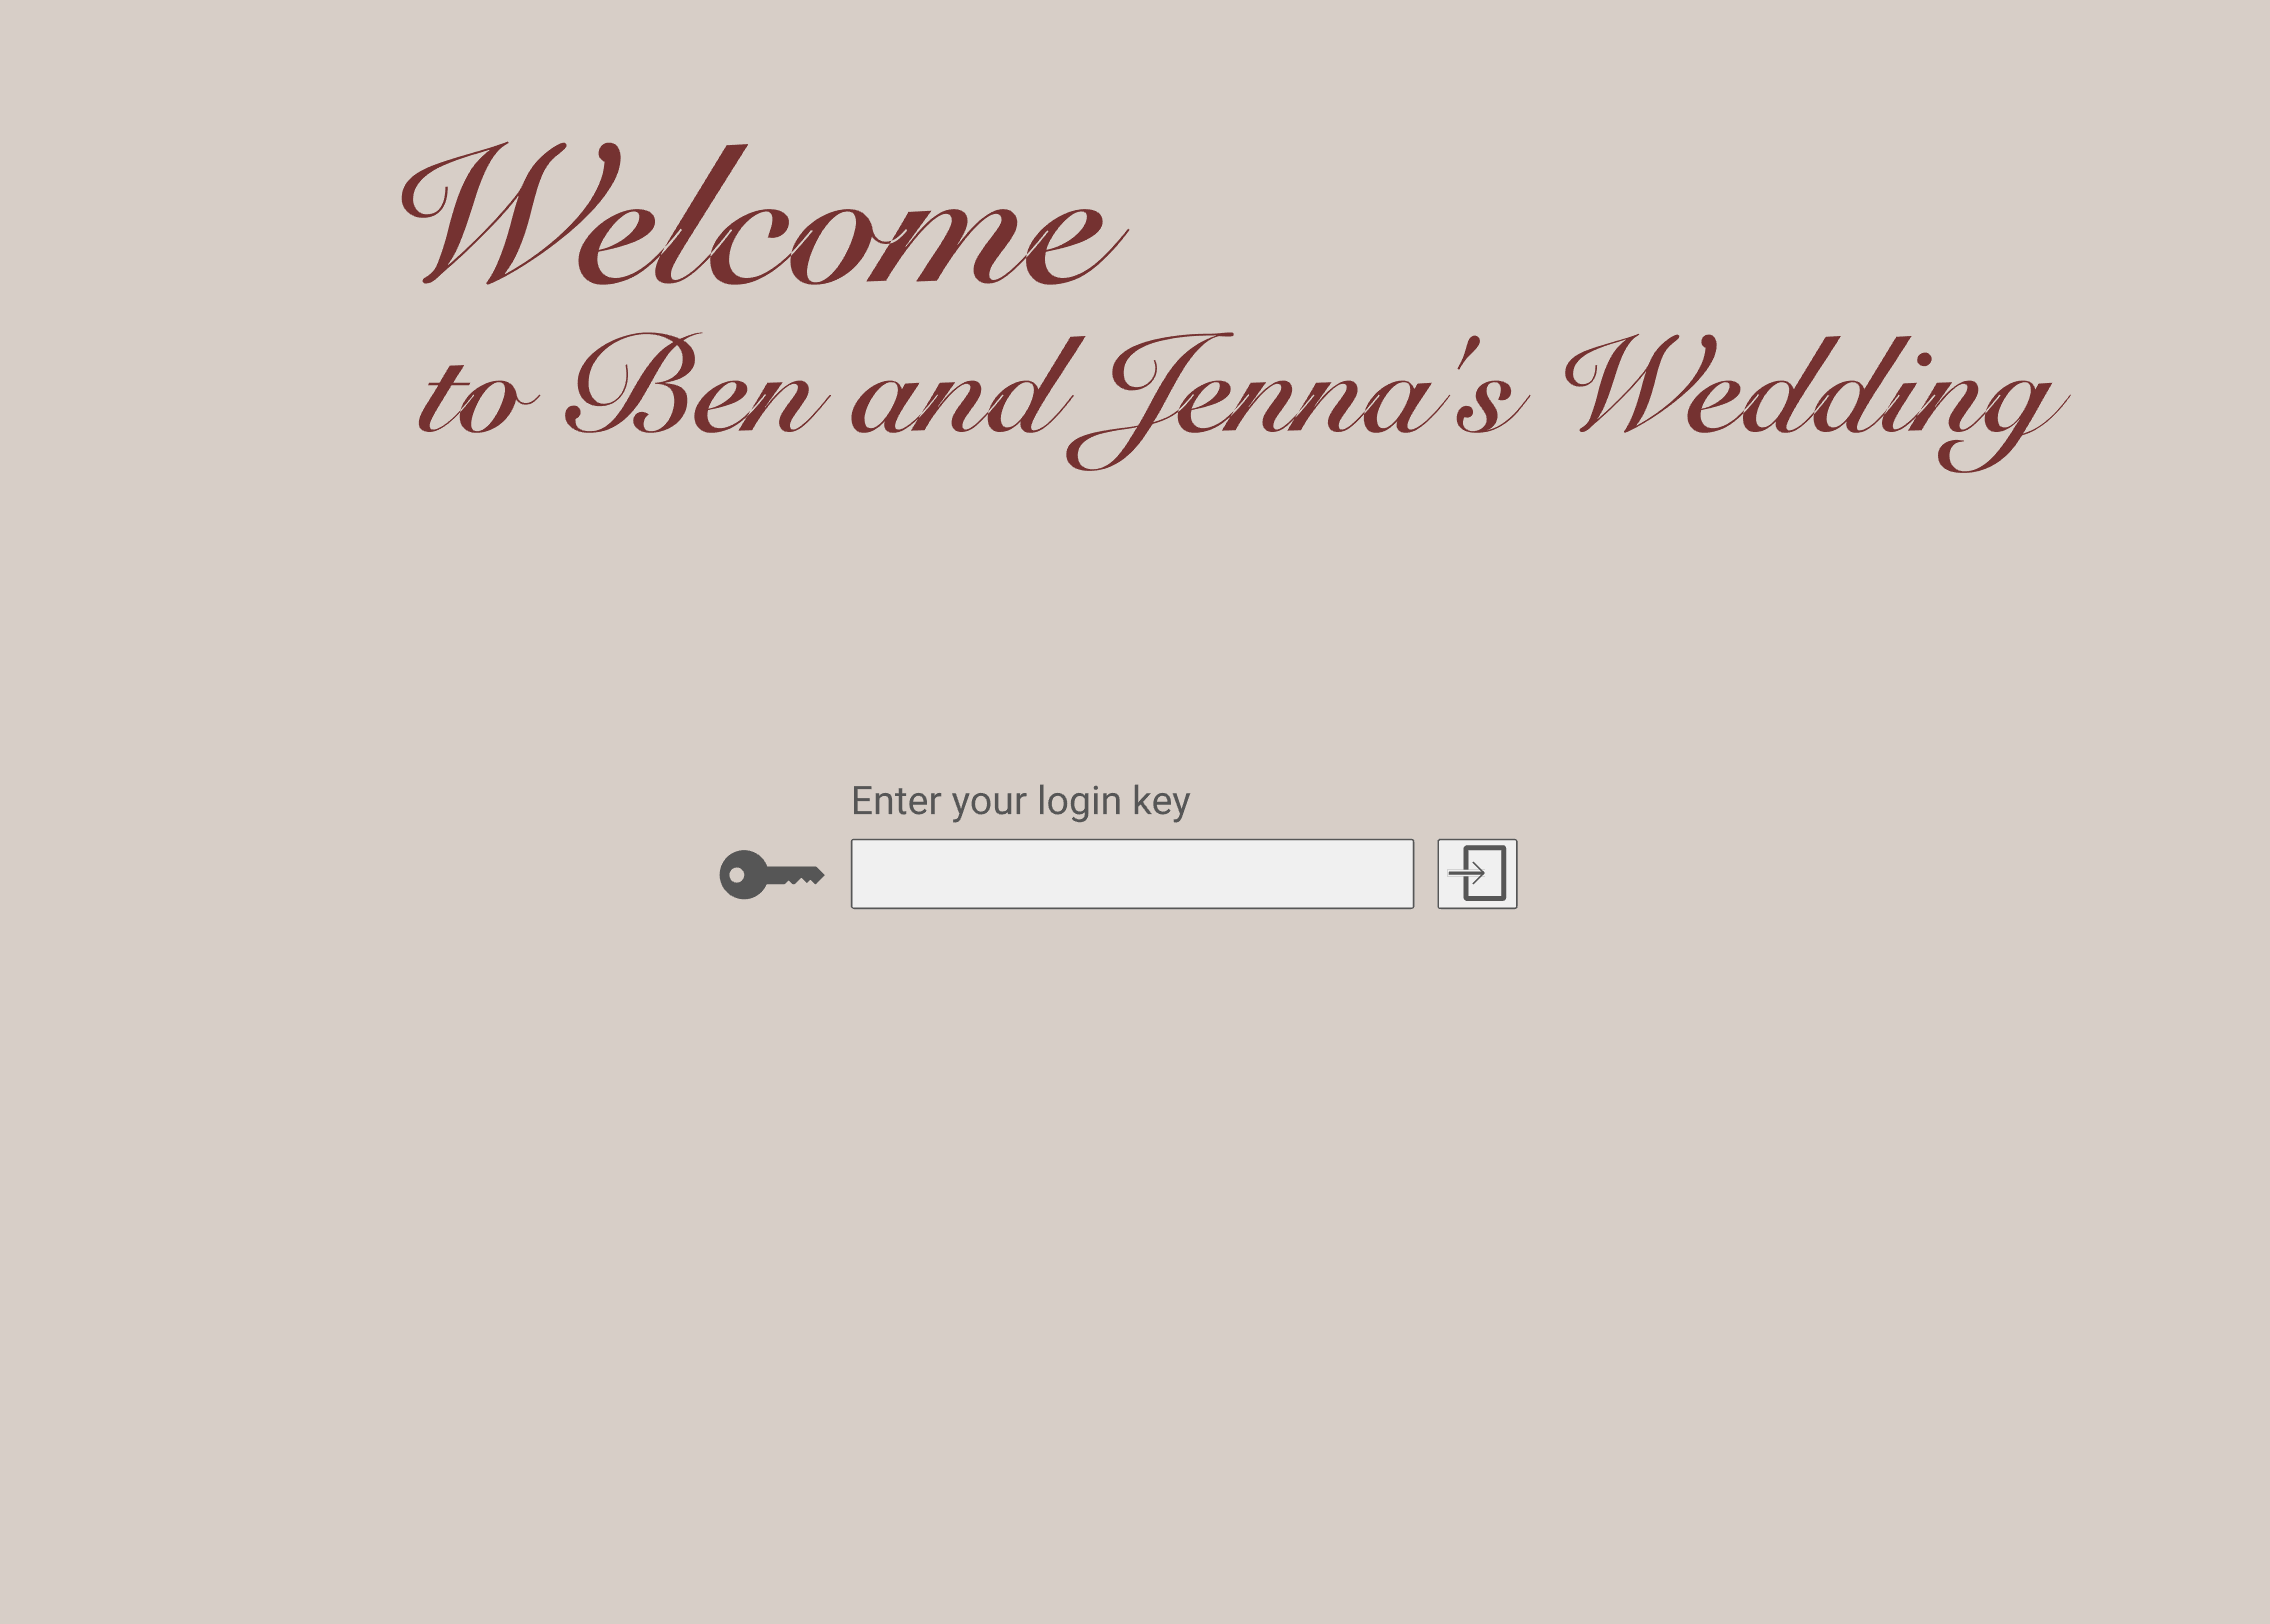
\includegraphics[width=0.8\linewidth]{Images/desktop-login.png} 
    \caption{The log-in screen.}
\label{fig1}
\end{figure}
2) To exit the viewer mode and return to the home page, select the logout option on the top right of the screen.
\subsubsection{View the stream}
1) To view the stream, select any icon that is visible from the venue image. \\
    \hspace*{1cm} a) If it is a regular stream, the viewer can watch the stream as it is displayed on the website. \\
    \hspace*{1cm} b) If it is a 360-degree stream, the viewer can either watch the stream regularly or they can select the view icon. 
    \hspace*{1cm} on the bottom right of the stream to enter the interactive 360-degree streaming mode. \\
2) To exit the stream, select either the back arrow on the top left of the video screen or the logout option on the top right \\ 
\hspace*{1cm} Note: selecting the logout option will return you to the homepage. 
\begin{figure}[h]%
    \centering
    \includegraphics[width=2.5in]{Images/website_pics/desktop-viewer.png}%
    \qquad
    \includegraphics[width=3in]{Images/website_pics/video_image.png}
    \caption{Viwer}
\end{figure}
\newpage
\subsection{Operation Guide - Admin}
1) On the homepage of the website, in the login section enter the token 'admin' and either press enter or select the icon to the immediate right of the login section. \\
2) To exit the admin mode and return to the home page, select the logout option on the top right of the screen. \\
\begin{figure}[h]
    \centering
    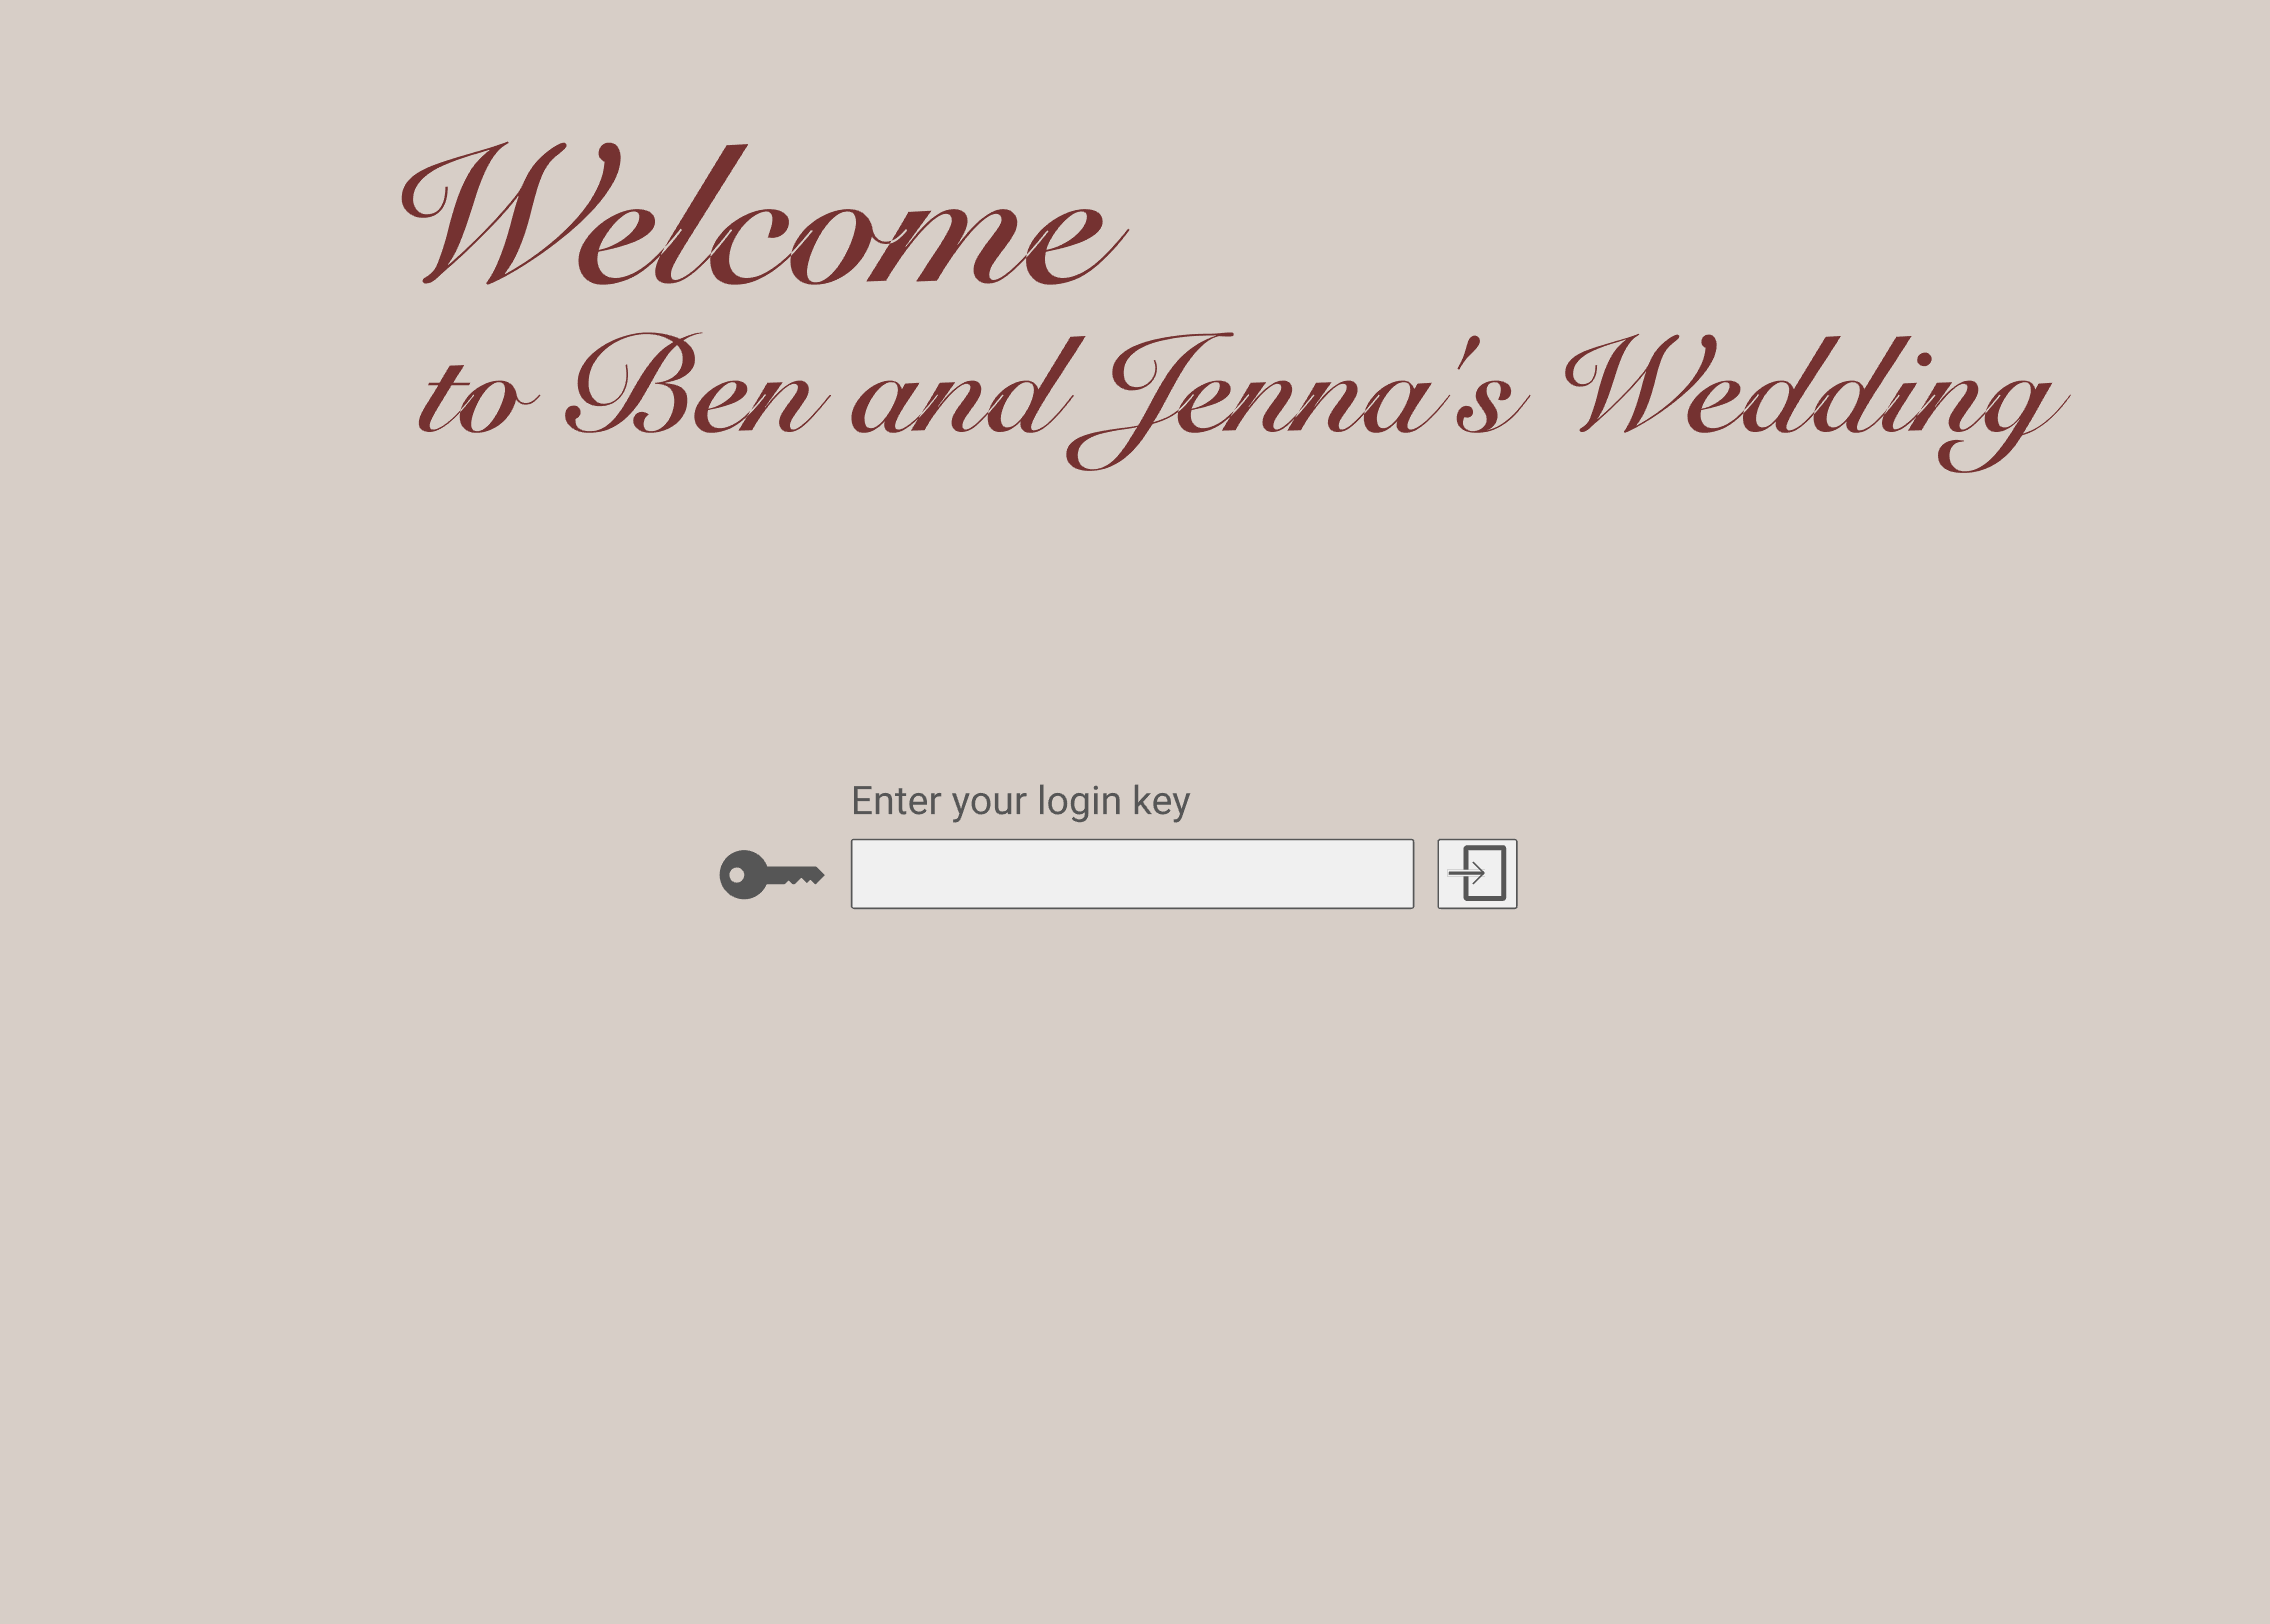
\includegraphics[width=0.8\linewidth]{Images/desktop-login.png} 
    \caption{Desktop log-in screen.}
\label{fig1}
\end{figure}
\subsubsection{View the stream}
1) To view the stream, select any icon that is visible from the venue image. \\
    \hspace*{1cm} a) If it is a regular stream, the viewer can watch the stream as it is displayed on the website. \\
    \hspace*{1cm} b) If it is a 360-degree stream, the viewer can either watch the stream regularly or they can select the view icon. \\
2) To exit the stream, select either the back arrow on the top left or the logout option on the top right. \\
\hspace*{1cm} Note: selecting the logout option will return you to the homepage.
\begin{figure}[h]%
    \centering
    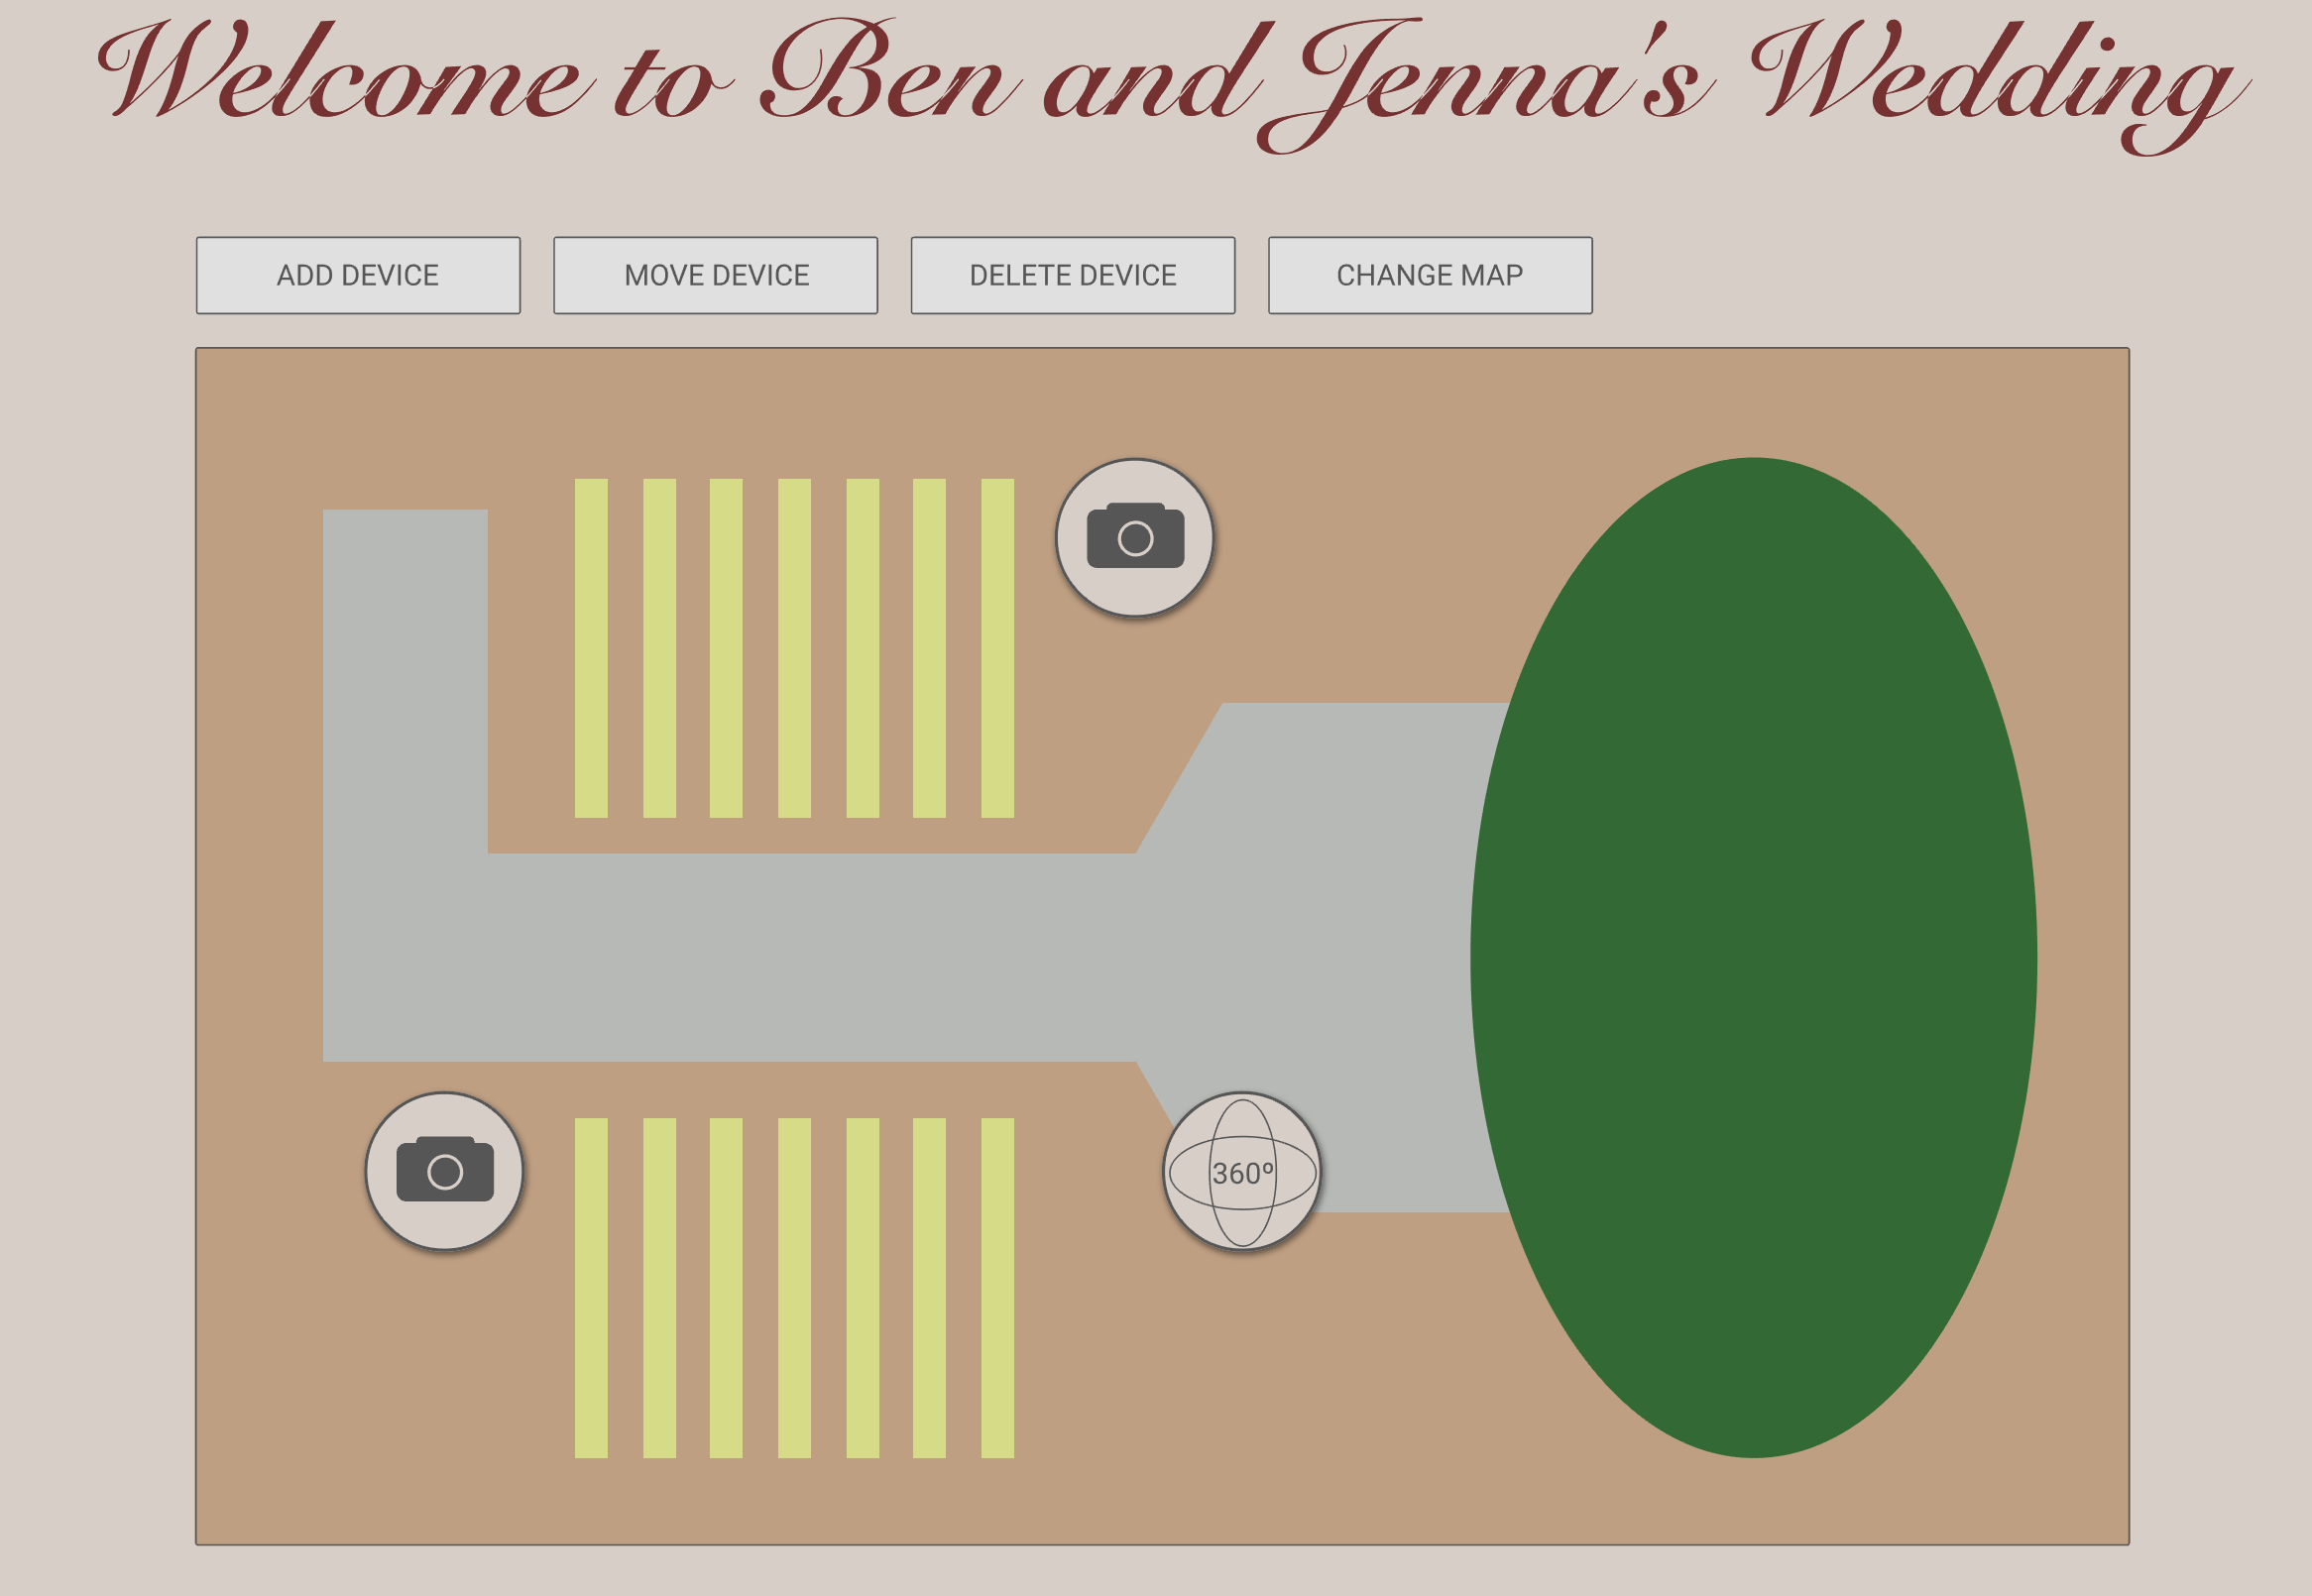
\includegraphics[width=2.5in]{Images/website_pics/desktop-admin.png}%
    \qquad
    \includegraphics[width=3in]{Images/website_pics/video_image.png}
    \caption{Desktop admin home view and video stream.}
\end{figure}
\newpage
\subsubsection{Add a device}
1) To add a device, select the 'ADD DEVICE' option on the top of the menu. \\
\hspace*{1cm} a) Device type: select the type of device you are adding from the following: \\
    \hspace*{2cm} - regular stream \\
    \hspace*{2cm} - 360-degree stream \\
    \hspace*{2cm} - an audio stream \\
\hspace*{1cm} b) Device name: this is the name you choose for your pi. \\ 
\hspace*{1cm} c) Device Code: this is the code you choose for your pi, please make sure this unique for each pi. \\
    \hspace*{2cm} Note: this will be used internally when the device icon is selected on the website. \\
\hspace*{1cm} d) Rows/Columns: the rows and columns you wish the dimensions of the grid to be. This will help with placing \hspace*{2cm } your pi on the map grid.\\
    \hspace*{2cm} Note: the rows and columns numbers must be positive integers.  \\
\hspace*{1cm} e) IP: enter the IP address of the raspberry pi you are connecting to. \\
\hspace*{2cm} Note: we put in the IP address of the router since we are port forwarding. \\
\hspace*{1cm} f) Port: enter the port number the raspberry pi is streaming to.
    \begin{itemize}
        \item Note: if there is an error with the format of any of the data entries, an error will pop up to direct the user to change their entry.
    \end{itemize}
\hspace*{1cm} Once the desired information is entered correctly, select 'submit' to add the device \\
\hspace*{1cm} or 'cancel' to exit the 'ADD DEVICE' window. 
\begin{figure}[h]
    \centering
    \includegraphics[width=0.8\linewidth]{Images/website_pics/add_device.PNG} 
    \caption{Add a device modal.}
\label{fig1}
\end{figure}
\newpage
\subsubseciton{Removing a device}
1) To remove a device, select the 'DELETE DEVICE' option on the top of the menu. \\
2) Select the name of the device you wish to delete from the drop-down menu and select 'submit' to remove the device or 'cancel' to exit the 'DELETE DEVICE' window.
\begin{figure}[h]
    \centering
    \includegraphics[width=0.8\linewidth]{Images/website_pics/delete_device.PNG} 
    \caption{Delete a device modal.}
\label{fig1}
\end{figure}
\subsubsection{Move a device}
1) To move a device, select the 'MOVE DEVICE' option on the top of the menu. \\
2) Select the icon of the device you wish to move. \\
\hspace*{1cm} a) All available spaces that the device can be moved to will turn green. \\
3) Select the space you wish to move the device on the map to relocate it.
\\
\hspace*{1cm} Note: if you wish to exit 'MOVE DEVICE' without changing the device locations \\
     \hspace*{1.5cm} select 'CANCEL MOVE' in the menu.
\begin{figure}[h]%
    \centering
    \includegraphics[width=3.3in]{Images/website_pics/start_move.PNG}%
    \qquad
    \includegraphics[width=3.3in]{Images/website_pics/move_select.PNG}
    \caption{Move a device with grid and available area to move to.}
\end{figure}
\newpage
\subsubsection{Change map}
1) To change the map, select the 'CHANGE MAP' option on the top of the menu. \\
2) Select the 'Choose File' option which brings up a file explorer to choose the file that you wish to replace your current map with. \\
3) Select the dimensions of the map by entering the number of rows and columns as positive integers. \\
\hspace*{1cm} Note: if no file is chosen then the current map's dimensions will be changed instead. \\
4) Select 'UPLOAD FILE' to update the map, or 'CANCEL' to exit.
\begin{figure}[h]
    \centering
    \includegraphics[width=0.8\linewidth]{Images/website_pics/change_map.PNG} 
    \caption{Change map modal with image file browser.}
\label{fig1}
\end{figure}
\subsection{Conclusion}
This concludes the tutorial for the A-frame live stream portal project.
\newpage
\section{Recommended Technical Resources for Learning More}

    \subsection{Helpful Websites}
        \begin{enumerate}
          \item https://github.com/iizukanao/picam
          \item https://aframe.io/
          \item http://www.tinkernut.com/portfolio/make-cheap-360-video-camera-raspberry-pi/
          \item https://stackoverflow.com/
          \item http://hamelot.io/visualization/using-ffmpeg-to-convert-a-set-of-images-into-a-video/
          
        \end{enumerate}

\section{Conclusions and Reflections}

    \subsection{Louis}
    \begin{itemize}
        \item What technical information did you learn?
        \begin{itemize}
            \item I learned how to use PHP and MySQL to build my own website, I had previously used it on an existing system, but have never built anything from scratch until recently. I also got more experience programming on/using raspberry pis. I learned quite a bit about audio and video encoding while setting up the streaming, unfortunately we ended up not using most of it.
        \end{itemize}
        \item What non-technical information did you learn?
        \begin{itemize}
            \item Mostly just more practice writing documentation and having meetings, my group got along fairly well, we didn't have any major conflicts among us. 
        \end{itemize}
        \item What have you learned about project work?
        \begin{itemize}
            \item Its more difficult to do when you have other stuff going on. I already had experience working on large projects from my MECOP internship, there is a huge difference between working on something for 8 hours a day and working on it as you have free time throughout the week.
        \end{itemize}
        \item What have you learned about project management?
        \begin{itemize}
            \item Unforeseen issues can add a lot of time to estimates, also hardware limitations mean you should have your project ready to test well before it's due. 
        \end{itemize}
        \item What have you learned about working in teams?
        \begin{itemize}
            \item Having regular meeting times is important, I felt like we did a good job as a team.
        \end{itemize}
        \item If you could do it all over, what would you do differently?
        \begin{itemize}
            \item Get working on the video streaming part of the project way earlier. This is where most of our issues arose and we only really started it half way through winter term.
        \end{itemize}
    \end{itemize}
    
    \subsection{Meghan}
    \begin{itemize}
        \item What technical information did you learn?
        \begin{itemize}
            \item I learned how to use a raspberry pi. 
            More specifically I learned how to stream and record videos from the device.
        \end{itemize}
        \item What non-technical information did you learn?
        \begin{itemize}
            \item I learned how to use LaTex and how to keep minutes for meetings efficiently.
        \end{itemize}
        \item What have you learned about project work?
        \begin{itemize}
            \item I learned that communication is key with project work and that nothing can get done properly unless everyone is on the same page.
        \end{itemize}
        \item What have you learned about project management?
        \begin{itemize}
            \item I learned that it is important to properly plan out the timetable of when you are planning on completing portions of your project which will help prevent rushing at the end. 
            It is also important to allow for unexpected setbacks when planning out your project.
        \end{itemize}
        \item What have you learned about working in teams?
        \begin{itemize}
            \item I have learned that even if there are setbacks and problems, if you have a great team dynamic then you can complete a project regardless of the obstacles. 
        \end{itemize}
        \item If you could do it all over, what would you do differently?
        \begin{itemize}
            \item I would make sure I knew exactly what was due when for every stage of the project.
        \end{itemize}
    \end{itemize}
    
    \subsection{Sarahi}
    \begin{itemize}
        \item What technical information did you learn?
        \begin{itemize}
            \item I learned how to work with a raspberry pi. I had never used one before so I learned how to set it up, install libraries, dependencies, and to configure settings. I also learned how to stream video using a media player over the same network. Then I learned how to stream video with different network this took learning how to port forward. I learned how to adjust the focal point of the pi camera. Also how to record sound and play it back with a microphone attached to the pi. After switching from a media player to using an API I learned how to stream audio and video using Picam.
        \end{itemize}
        \item What non-technical information did you learn?
        \begin{itemize}
            \item During this project a reoccurring theme that would pop up was that often following tutorials was not enough. I learned that often it would take just one small detail that was missing to make things work. So I learn that a lot of engineering is searching through information to find something that is useful and even when you find it, it may not be complete so look some more.
        \end{itemize}
        \item What have you learned about project work?
        \begin{itemize}
            \item I learned that project work is long, and tedious, but rewarding.
        \end{itemize}
        \item What have you learned about project management?
        \begin{itemize}
            \item I learned that project management is not that hard when the people involved are invested and care to do well like in our case.
        \end{itemize}
        \item What have you learned about working in teams?
        \begin{itemize}
            \item  There was not much new I learned from working in a team. However the takeaway is that the people that make up the team greatly determine the success of the project. 
        \end{itemize}
        \item If you could do it all over, what would you do differently?
        \begin{itemize}
            \item If I could start over I would have been more careful of selecting what tutorials to follow. There was time wasted following tutorial that were a stepping stone to better methods. It was not a complete waste of time but for example instead of following tutorials to stream video, then tutorials to stream audio, I  would have searched and used instead a tutorial that had both. A lot of work was stepping stones to the final solution so if I could start over I would skip those to the useful ones right off the bat to save time but it was a learning experience. 

        \end{itemize}
    \end{itemize}

\section{Appendix 1: Essential Code listings}

\begin{lstlisting}
def buildMap(finalImageWidth,finalImageHeight,innerRadius,outerRadius,centerX,centerY):
    map_x = np.zeros((int(finalImageHeight),int(finalImageWidth)),np.float32)
    map_y = np.zeros((int(finalImageHeight),int(finalImageWidth)),np.float32)
    rMap = np.linspace(innerRadius, innerRadius + (outerRadius - innerRadius), finalImageHeight)
    thetaMap = np.linspace(0, 0 + float(finalImageWidth) * 2.0 * np.pi, finalImageWidth)
    sinMap = np.sin(thetaMap)
    cosMap = np.cos(thetaMap)
    for y in xrange(0, int(finalImageHeight-1)):
       map_x[y] = centerX + rMap[y] * sinMap
       map_y[y] = centerY + rMap[y] * cosMap
    return map_x, map_y
\end{lstlisting}

A circular image is captured by the camera using the 360 lens and is then converted to a rectangular image. The code snippet above remaps the image using a center point, an inner radius, and an outer radius. The map is built once and then the xmap and ymap values are used for the openCV remap function.

\begin{lstlisting}
output = cv2.remap(img,xmap,ymap,cv2.INTER_LINEAR)
\end{lstlisting}
Which gives up a dewarped frame that we can use to make a video.


\section{Appendix 2: Figures}

    \begin{figure}[!hb]
        \centering
        \includegraphics[scale=0.3]{Images/UML_Diagram.png}
        \centering\caption{System Architecture UML Diagram.}
        \label{fig:Architecture}
    \end{figure}

%desktop pictures

 \begin{figure}[h!]
            \centering
            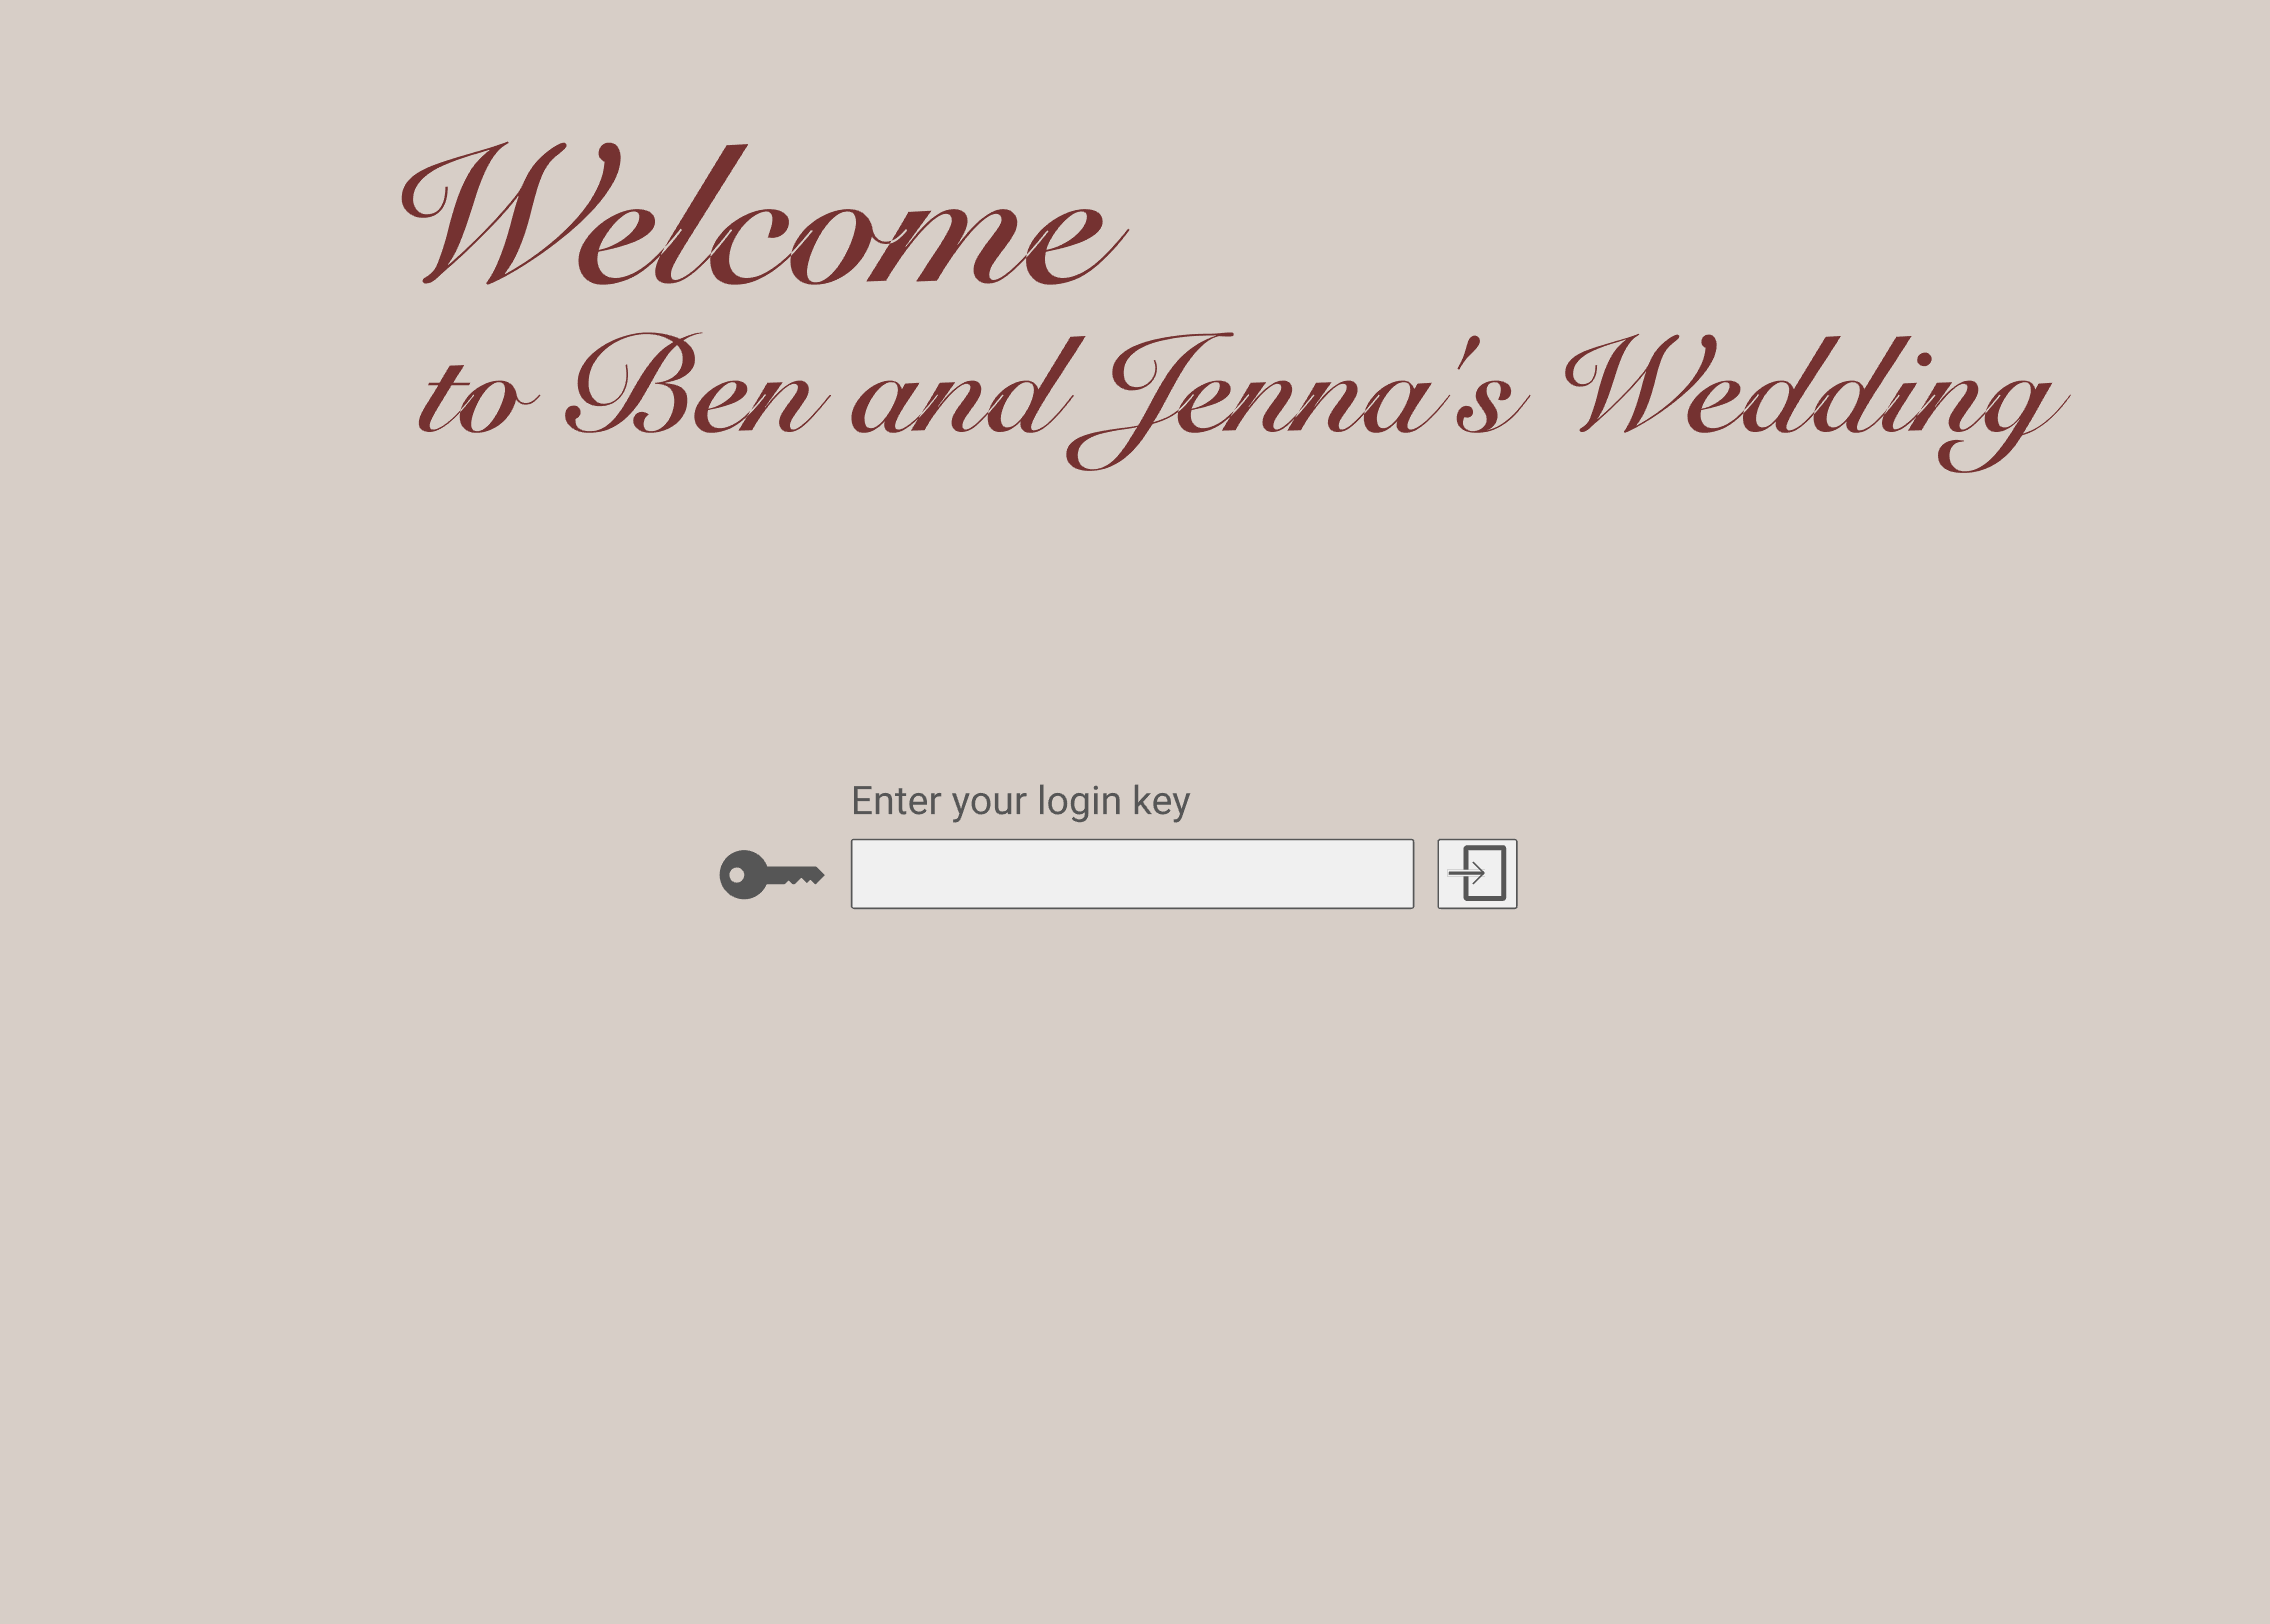
\includegraphics[scale=0.4]{Images/desktop-login.png}
            \centering\caption{Login Page}
            \label{fig:Login}
        \end{figure}
        
        \begin{figure}[h!]
            \centering
            \includegraphics[scale=0.17]{Images/website_pics/desktop-viewer.png}
            \centering\caption{User View Homepage}
            \label{fig:User}
        \end{figure}
        \begin{figure}[h!]
            \centering
            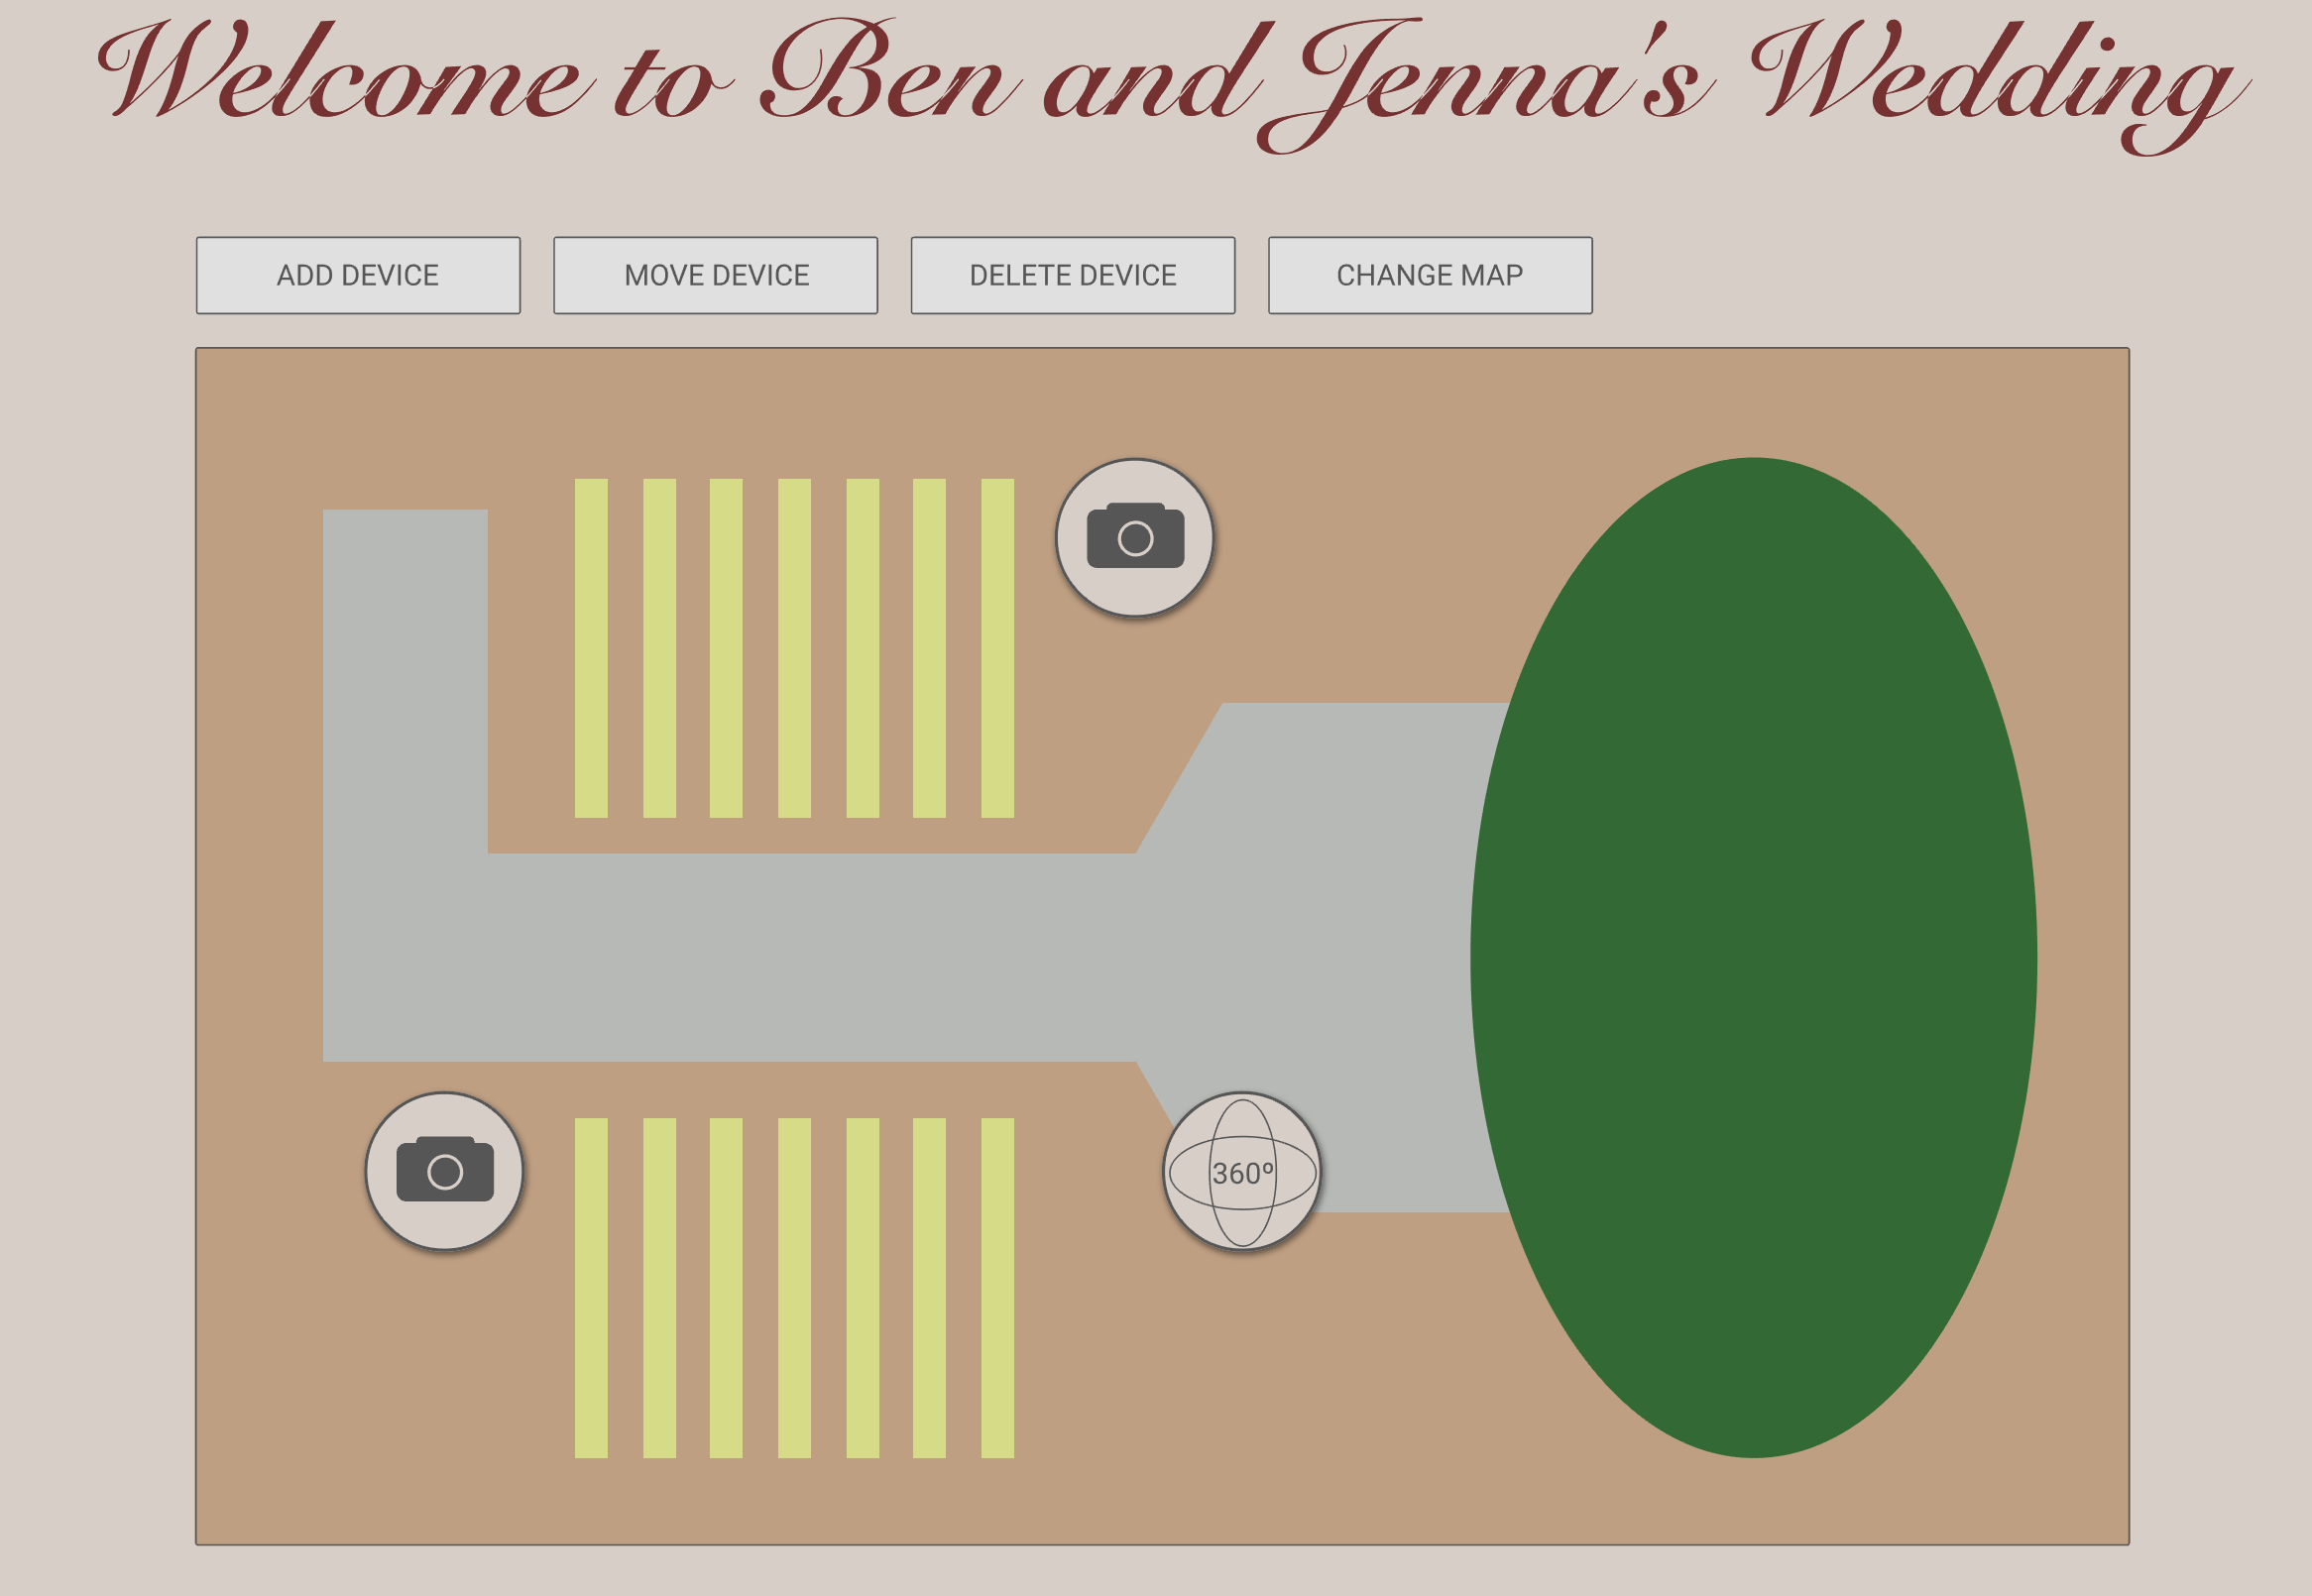
\includegraphics[scale=0.17]{Images/website_pics/desktop-admin.png}
            \centering\caption{Admin View Homepage}
            \label{fig:Admin}
        \end{figure}
        
        \begin{figure}[h!]
            \centering
            \includegraphics[scale=0.35]{Images/website_pics/video_image.png}
            \centering\caption{Video Stream Page}
            \label{fig:Video}
        \end{figure}



%MOBILE pictures    
   
    \begin{figure}[h!]
        \centering
        \includegraphics[scale=0.3]{Images/website_pics/mobile/login_mobile.jpg}
        \centering\caption{Mobile Login Page}
        \label{fig:MLogin}
    \end{figure}
    
    \begin{figure}[h!]
        \centering
        \includegraphics[scale=0.3]{Images/website_pics/mobile/viewer_mobile.jpg}
        \centering\caption{Mobile User View Homepage}
        \label{fig:MUser}
    \end{figure}
    
    \begin{figure}[h!]
        \centering
        \includegraphics[scale=0.3]{Images/website_pics/mobile/admin_mobile.jpg}
        \centering\caption{Mobile Admin View Homepage}
        \label{fig:MAdmin}
    \end{figure}

    \begin{figure}[h!]
        \centering
        \includegraphics[scale=0.3]{Images/website_pics/mobile/video_mobile.jpg}
        \centering\caption{Mobile Video Page}
        \label{fig:MVideo}
    \end{figure}

\end{document}
